% !TeX root = ../HebutThesis_example.tex(此文件是被HebutThesis_example.tex调用的)
\chapter{基本理论与方法}




\section{生成模型介绍}
生成模型可以通过在数据集上训练,学习数据集中样本的概率分布{$p_{data}$},
用生成模型所获得的{$p_{model}$}来近似{$p_{data}$},
训练完成获得{$p_{model}$}之后,可以通过从{$p_{model}$}中采样来生成与数据集中相似的样本。

生成模型不仅仅可以应用在近些年有较大突破的图片生成与聊天机器人,还包括很多更广泛的应用{ {\cite{goodfellow2016nips}}},如:

\begin{itemize}
    \item 生成模型的训练和采样,有助于表示和运用高维度概率分布。高维度概率分布在数学和工程领域应用广泛。
    \item 生成模型可以与强化学习相结合,如进行未来决策或对环境的模拟。
    \item 生成模型可以辅助半监督学习,如对无标签数据进行标注。
    \item 生成模型可以应用于多模态领域,如对同一输入,不仅仅生成文字,同时也可以生成图像。
    \item 从本质上来说,很多任务都需要从一些概率分布中进行采样,如提高图像分辨率,艺术创作,图像与图像之间的转换等。
\end{itemize}

很多生成模型应用极大似然估计的原理。
极大似然估计的基本思想是,
定义一个由参数{$\bm{\theta}$}确定的对概率分布的估计{$p_{model}(\bm{x};\bm{\theta})$},
之后,对训练集定义似然函数

\begin{equation}
    \label{eq:likelihood_for_training_data}
    \prod_{i=1}^{m}{p_{model}({\bm{x}}^{(i)};\bm{\theta})}
\end{equation}


式{\ref{eq:likelihood_for_training_data}}中,
{$m$}为该训练集样本数,
{$\bm{x}^{(i)}$}为训练集中样本。
\begin{align}
    \bm{\theta}^{*}
        & = \argmax_{\bm{\theta}}{\prod_{i=1}^{m}{p_{model}({\bm{x}}^{(i)};\bm{\theta})}} \label{eq:theta_star_max_1} \\
        & = \argmax_{\bm{\theta}}{\log{\prod_{i=1}^{m}{p_{model}({\bm{x}}^{(i)};\bm{\theta})}}} \label{eq:theta_star_max_2} \\
        & = \argmax_{\bm{\theta}}{{\sum_{i=1}^{m}{\log p_{model}({\bm{x}}^{(i)};\bm{\theta})}}} \label{eq:theta_star_max_3}  
\end{align}


选取参数{$\bm{\theta}^*$}使似然函数式{\ref{eq:likelihood_for_training_data}},取得最大值,
为方便计算,相比于将原似然函数进行最大化,可以将其转化之对数空间,这样可以将求积变为求和。
在式{\ref{eq:theta_star_max_2}}中,应用了对数函数为单调递增函数,不改变参数最大值取值的性质。
获得的生成模型即为{$p_{model}(\bm{x};\bm{\theta})$}。
图{\ref{fig:max_likelihood}}展示了一维极大似然估计过程,
极大似然估计从训练集中采样,
增大样本所在位置概率的同时保证概率密度总积分为1。

\begin{figure}[ht]
    \centering
    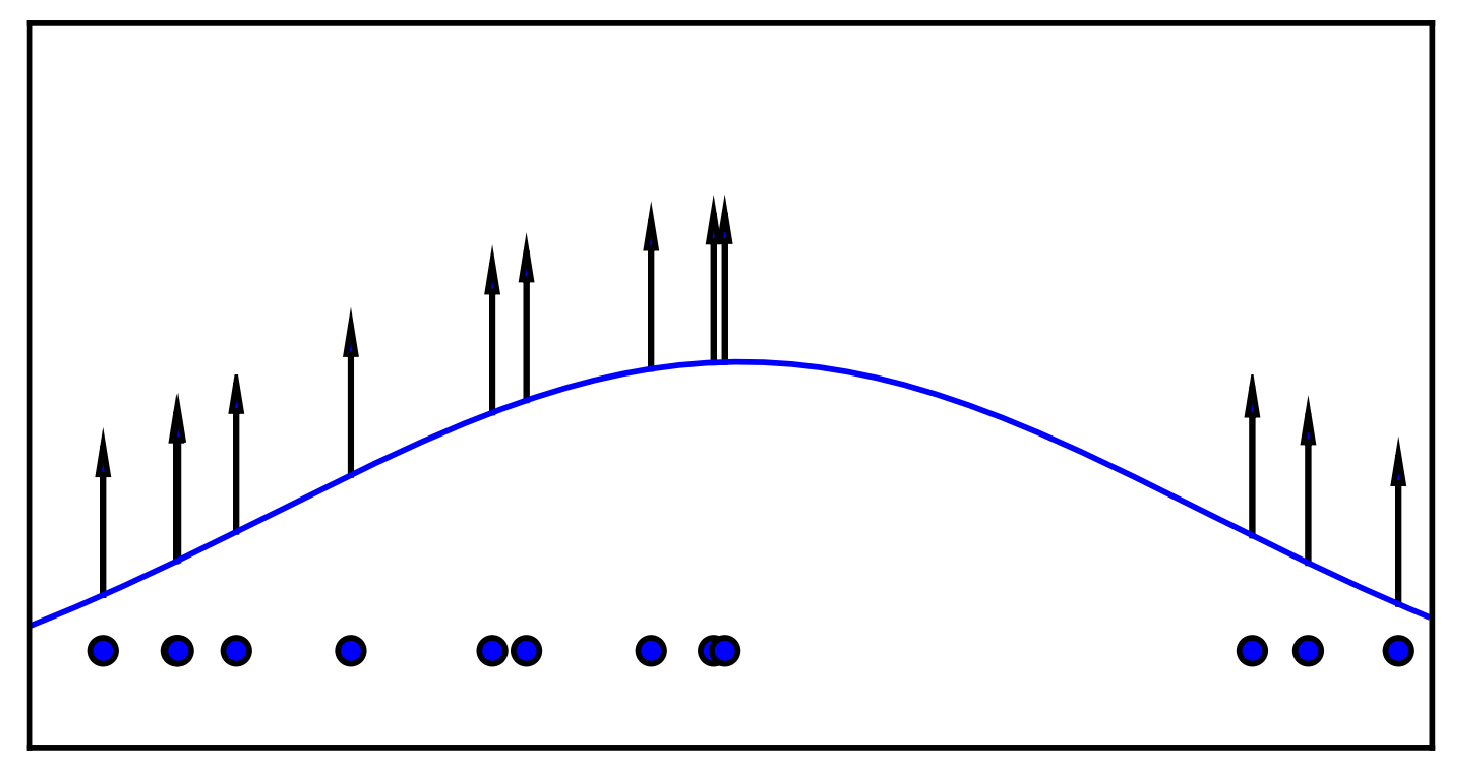
\includegraphics[width=0.8\textwidth]{figures/max_likelihood}
    \caption{一维极大似然估计过程}\label{fig:max_likelihood}
\end{figure}

从另一方面来说,
对参数{$\bm{\theta}^*$}进行极大似然估计与最小化生成模型与样本数据的实际概率分布的KL散度等价,
即:
\begin{equation}
    \label{eq:kl_divergence_max_theta}
    \bm{\theta}^{*}=\argmax_{\bm{\theta}}{D_{KL}{(p_{data}(\bm{x})||p_{model}(\bm{x};\bm{\theta}))}}
\end{equation}

可以根据如何表示或近似似然函数对生成模型进行分类。
具体地说,主要可以分为以下三类:
\begin{itemize}
    \item 可求解的显示密度模型,直接定义概率密度函数{$p_{model}(\bm{x};\bm{\theta})$},且要求其似然函数可直接求解。如规范化流模型和自回归模型。
    \item 近似估计的显示密度模型,直接定义概率密度函数{$p_{model}(\bm{x};\bm{\theta})$},且要求其似然函数可求得近似解。如基于能量的模型、变分自编码器和扩散模型。
    \item 隐式密度模型,不定义概率密度函数,而通过其他间接方式对概率分布{$p_{data}$}进行学习。如生成对抗网络。
\end{itemize}


\section{显式密度模型}\label{section:explicit_density_model}
显式密度模型直接定义概率密度函数{$p_{model}(\bm{x};\bm{\theta})$},之后即可以根据极大似然估计进行模型拟合。
显式密度模型存在的主要问题是:很难设计既可以表示样本分布又容易求解的模型。
有两种方法可以解决这个问题:
\begin{enumerate}
    \item 设计易求解的模型结构,在此基础上提高模型表达能力,即可求解密度模型。
    \item 设计模型后,通过近似方法求解似然函数,即近似估计密度模型。
\end{enumerate}


\subsection{可求解密度模型}
\subsubsection{规范化流模型}

规范化流模型通过一系列可逆变换方程,
将简单的概率分布逐渐转化为复杂的概率分布,
以希望能够拟合数据样本的概率分布。

\begin{figure}[ht]
    \centering
    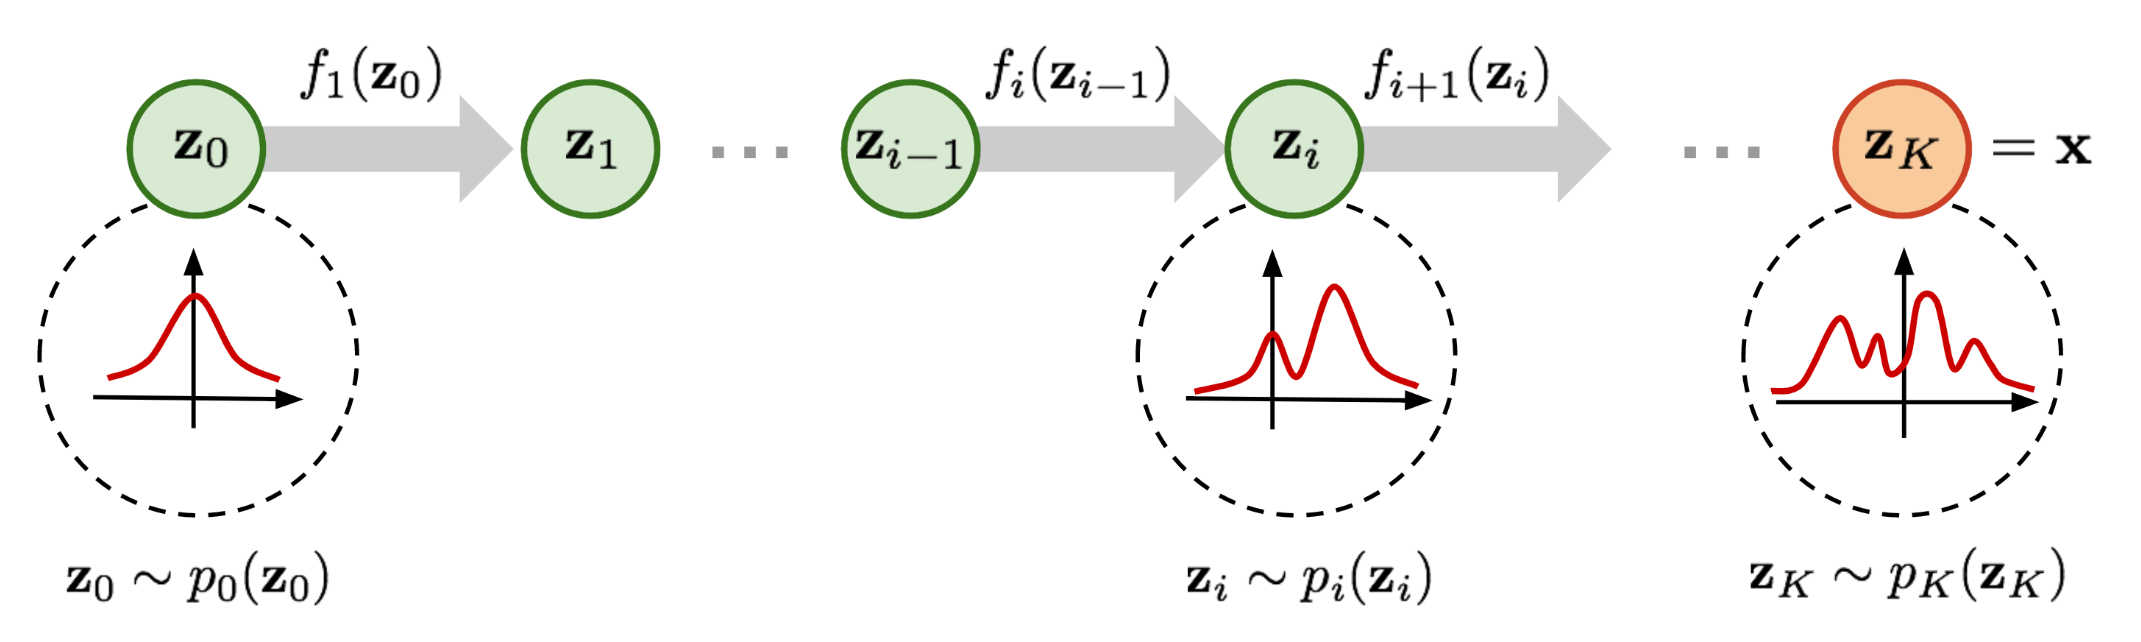
\includegraphics[width=0.8\textwidth]{figures/normalizing_flow}
    \caption{规范化流模型示意图}\label{fig:normalizing_flow}
\end{figure}
如图{\ref{fig:normalizing_flow}}所示,
\begin{align}
    \bm{z}_{i-1} &\thicksim p_{i-1}(\bm{z}_{i-1}) \\
    \bm{z}_i&=f_i(\bm{z}_{i-1})
\end{align}
由反函数定理,
\begin{equation}
    \bm{z}_{i-1}=f_{i}^{-1}(\bm{z}_i)
\end{equation}
由附录式{\ref{eq:mutivariable_change_variable_in_probability}},
\begin{equation}
    \label{eq:normalizing_flow_p_of_z}
    p_i(\bm{z}_i)=p_{i-1}(f_i^{-1}(\bm{z}_i))\left\rvert \det \frac{df_i^{-1}}{d\bm{z}_i}\right\rvert
\end{equation}
为获得{$p_i(\bm{z}_i)$}与{$p_{i-1}(\bm{z}_{i-1})$}之间的关系,
对式{\ref{eq:normalizing_flow_p_of_z}}进行变形:
\begin{align}
    p_i(\bm{z}_i)
    & = p_{i-1}(f_i^{-1}(\bm{z}_i))\left\rvert \det\frac{df_{i}^{-1}}{d\bm{z}_i} \right\rvert \\
    & = p_{i-1}(\bm{z}_{i-1})\left\rvert \det {(\frac{df_{i}}{d\bm{z}_{i-1}})}^{-1} \right\rvert &\mbox{(根据式{\ref{eq:inverse_function_theorem_application}})}\\
    & = p_{i-1}(\bm{z}_{i-1})\left\rvert \det \frac{df_{i}}{d\bm{z}_{i-1}} \right\rvert^{-1}  &\mbox{(根据式{\ref{eq:determinant_of_inverse_matrix}})} \label{eq:normalizing_flow_change_variable}
\end{align}
对式{\ref{eq:normalizing_flow_change_variable}}进行对数化得:
\begin{equation}
    \label{eq:normalizing_flow_flow_equation}
    \log p_i(\bm{z}_i)=\log p_{i-1}(\bm{z}_{i-1})-\log \left\rvert \det \frac{df_{i}}{d\bm{z}_{i-1}}   \right\rvert
\end{equation}
连续应用式{\ref{eq:normalizing_flow_flow_equation}},
对{$\bm{x}$}不断变换可得其关于简单概率分布变量{$\bm{z}$}的表达式,即:
\begin{align}
    \bm{x}=\bm{z}_K 
    & =f_K\circ f_{K-1} \circ \cdots  \circ f_1(\bm{z}_0) \\
    \log p(\bm{x})= \log p_K(\bm{z}_K)
    & =\log p_{K-1}(\bm{z}_{K-1}) - \log \left| \det \frac{df_K}{d\bm{z}_{K-1}} \right| \\
    & =\log p_{K-2}(\bm{z}_{K-2}) - \log \left| \det \frac{df_{K-1}}{d\bm{z}_{K-2}} \right| - \log \left| \det \frac{df_K}{d\bm{z}_{K-1}} \right| \\
    & = \cdots \\
    & = \log p_0(\bm{z}_0) - \sum_{i=1}^{K} \log \left| \det \frac{df_i}{d\bm{z}_{i-1}}\right|
\end{align}

所谓规范化流模型中的流指的是一系列随机变量之间的代换,
即不断应用{$\bm{z}=f_i(\bm{z}_{i-1})$}。
规范化流是指由一系列分布{$p_i$}组成的完整链式过程{ {\cite{weng2018flow}}}。

由上述计算过程,转换函数{$f_i$}需要满足两个条件:
\begin{itemize}
    \item 具备可逆性质;
    \item 雅可比矩阵容易计算。
\end{itemize}

\subsubsection{自回归模型}

自回归模型将生成问题简化成顺序问题,即通过之前的顺序值来预测下一个值。
一般来说,自回归模型对于高维数据{$x$}将其联合概率分布化为条件概率的乘积的形式:
\begin{equation}
    \label{eq:autoregressive_model_defination}
    p(\bm{x})=p(x_1,\ldots ,x_n)=\prod_{i=1}^{n}p(x_i|x_1,\ldots ,x_{i-1})
\end{equation}
对条件概率的模拟比直接对联合概率分布进行建模更加容易。

具体而言,为便于求解可以假定每一个变量只依赖于不超过一定数量的变量,比如两个变量,即:
\begin{equation}
    p(\bm{x})=p(x_1)p(x_2|x_1)\prod_{d=3}^{D}p(x_d \vert x_{d-1},x_{d-2})
\end{equation}

\begin{figure}[ht]
    \centering
    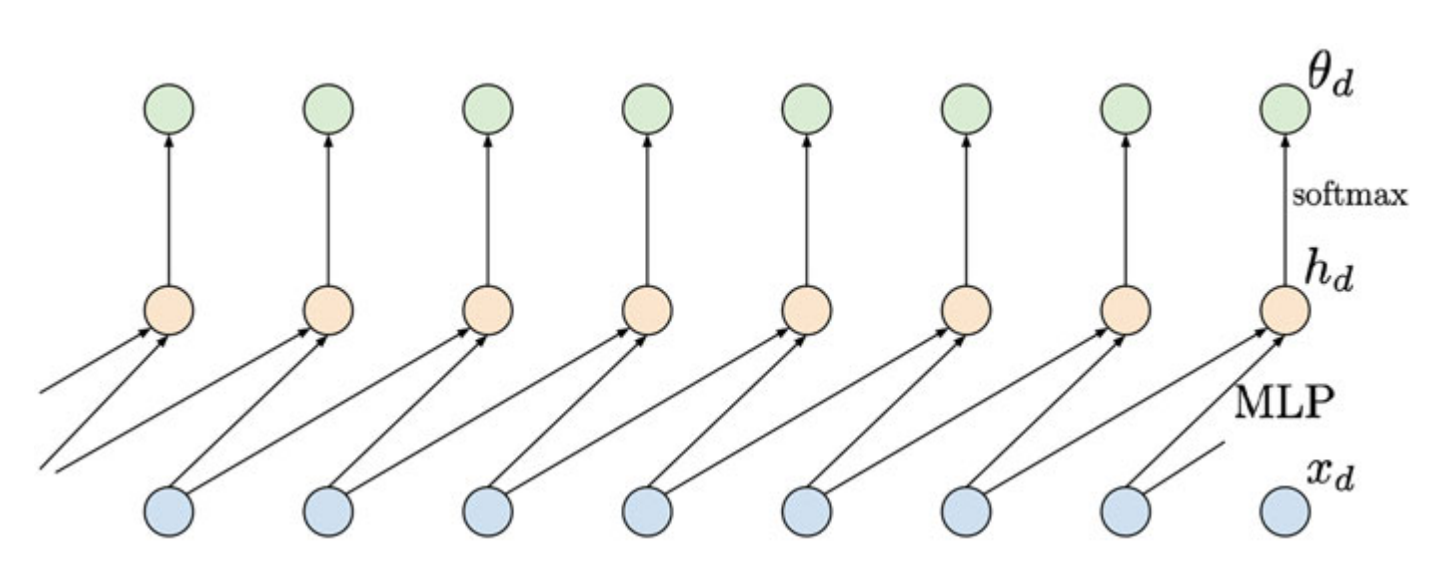
\includegraphics[width=0.8\textwidth]{figures/autoregressive_model_finite_memory}
    \caption{自回归模型依赖两变量示意图}\label{fig:autoregressive_model_finite_memory}
\end{figure}
可以使用多层感知机预测{$x_d$}的概率分布,
图{\ref{fig:autoregressive_model_finite_memory}}表示使用多层感知机进行预测{$x_d$}的概率分布。
最下面的蓝色结点表示输入,
中间层橘色结点表示多层感知机对前两个数据处理后的输出,
最后绿色点表示通过归一化指数函数输出的概率{$p(x_d \rvert x_{d-1},x_{d-2})$},即{$\theta_d$}。
但是,这种假设,即每一个变量只依赖于不超过一定数量的变量,对模型造成了很大的限制。
通过循环神经网络可以对以往信息进行更长期的保存{ {\cite{Jakub2022deep}}},即:
\begin{equation}
    \label{eq:autoregressive_model_rnn}
    p(x_d \rvert \bm{x}_{<d})=p(x_d \vert RNN(x_{d-1},h_{d-1}))
\end{equation}

式{\ref{eq:autoregressive_model_rnn}}中,
{$h_d=RNN(x_d, h_{d-1})$},{$h_d$}可以看作对所有历史信息的保存,可称为隐环境。
图{\ref{fig:autoregressive_model_rnn}}表示使用循环神经网络RNN预测{$x_d$}的概率分布。
最下面的蓝色结点表示输入,
中间层橘色结点表示循环神经网络对前两个输入数据与隐环境处理后的输出,
最后绿色结点表示通过归一化指数函数后输出的概率{$p(x_d \rvert x_{d-1},x_{d-2})$},即{$\theta_d$}。
\begin{figure}[ht]
    \centering
    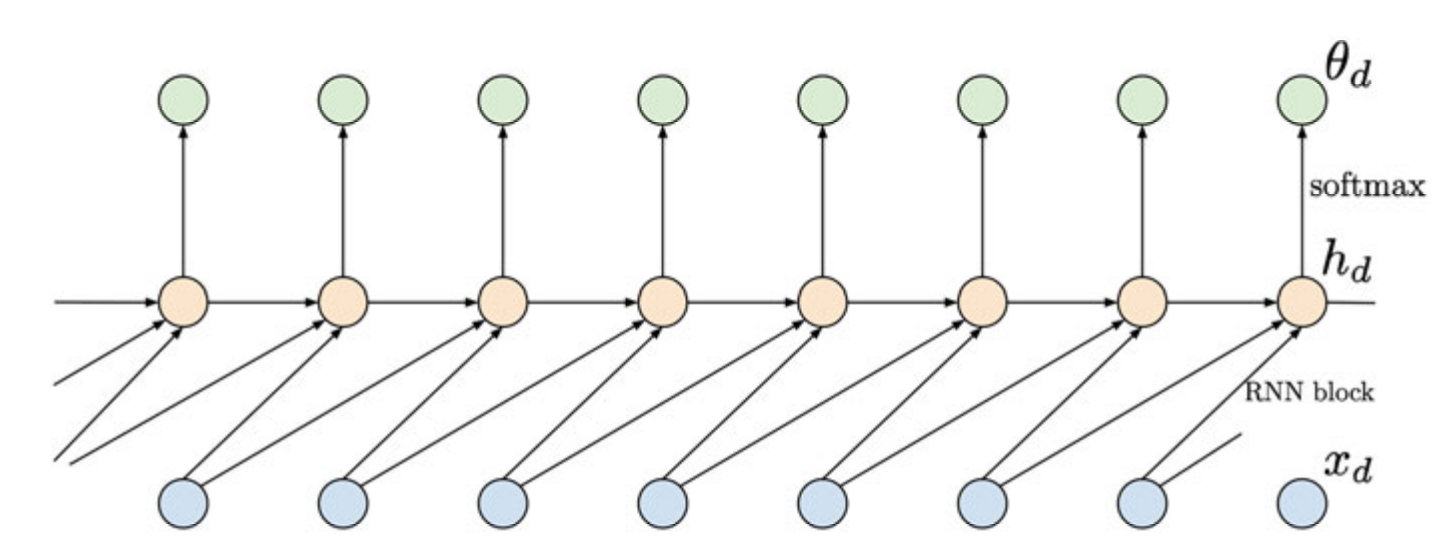
\includegraphics[width=0.8\textwidth]{figures/autoregressive_model_rnn}
    \caption{循环神经网络示意图}\label{fig:autoregressive_model_rnn}
\end{figure}

此外,transformer也属于自回归模型,transformer通过自注意力机制来对历史信息进行处理。


\subsection{近似估计密度模型}
\subsubsection{基于能量的模型}
%玻尔兹曼机
%Contrastive Divergence
%Langevin Dynamics
基于能量的模型的诞生受到对物理系统建模的启发——
一个事件的概率可以由玻尔兹曼分布式{\ref{eq:boltzmann_equation}}表示{\cite{lippe2022uvadlc}}。
如果一个神经网络{$E_{\theta}(\bm{x})$}只有一个输出神经元,
{$\theta$}表示神经网络的参数,
{$\bm{x}$}表示神经网络的输入,
其输出结果为实值标量,
那么有:
\begin{equation}
    \label{eq:energy_based_model_probability}
    q_{\theta}(\bm{x})=\frac{\exp(-E_{\theta}(\bm{x}))}{Z_{\theta}}
    \mbox{ ,其中}
    Z_{\theta}=
    \begin{cases}
        \int_{\bm{x}} \exp(-E_{\theta}(\bm{x})) \,d\bm{x}  & \bm{x}\mbox{为连续变量}\\
        \sum_{\bm{x}}\exp(-E_{\theta}(\bm{x}))       & \bm{x}\mbox{为离散变量}
    \end{cases}
\end{equation}

式{\ref{eq:energy_based_model_probability}}中,
指数函数保证所得概率大于0,
在{$E_{\theta}(\bm{x})$}前添加负号以表示{$E_{\theta}$}为能量函数:
样本点概率取值越高则其能量越低,
概率取值越低则具有更高的能量。
{$Z_{\theta}$}是归一化项用来保证概率密度积分或和为1,
如式{\ref{eq:energy_based_model_integrates_sum_to_1}}所示:
\begin{equation}
    \label{eq:energy_based_model_integrates_sum_to_1}
    \int_{\bm{x}} q_{\theta}(\bm{x}) \,d\bm{x} 
    = \int_{\bm{x}} \frac{\exp(-E_{\theta}(\bm{x}))}{\int_{\bm{\hat{x}}} \exp(-E_{\theta}(\bm{\hat{x}})) \,d\bm{\hat{x}}} \,d\bm{x}
    =\frac{\int_{\bm{x}} \exp(-E_{\theta}(\bm{x})) \,d\bm{x}}{\int_{\bm{\hat{x}}} \exp(-E_{\theta}(\bm{\hat{x}})) \,d\bm{\hat{x}}}
    =1
\end{equation}

式{\ref{eq:energy_based_model_probability}}与式{\ref{eq:energy_based_model_integrates_sum_to_1}}中,
{$q_{\theta}(\bm{x})$}为{$p(\bm{x})$}的近似,通过训练,可以使{$q_{\theta}(\bm{x})$}逐渐接近{$p(\bm{x})$}。

对于基于能量的模型,
{$E_{\theta}$}可以根据需要灵活选择。
由于归一化常数{$Z_{\theta}$}未知,
无法直接计算对数似然函数,
且由于{$Z_{\theta}$}不一定能保证不变,
不可直接对未进行归一化的概率{$\exp(-E_{\theta}(\bm{x}_{train}))$}极大化,
即不一定保证训练样本点相比其他数据点有更高的概率出现。
对于极大似然函数的计算,可以通过对比散度方法来进行近似。
通过比较不同数据点的似然来进行计算,
根据附录式{$\ref{eq:contrastive_divergence_partial_negative_log_likelihood}$}可得负对数似然函数,
\begin{align}
    \nabla _{\theta} Loss(q_{\theta}(\bm{x}))
    &= - \mathbb{E}_{p(\bm{x})}\left[ \nabla_{\theta} \log q_{\theta}(\bm{x}) \right] \label{eq:energy_based_model_nnl_origin} \\
    &= \mathbb{E}_{p(\bm{x})}\left[ \nabla_{\theta} E_{\theta}(\bm{x}) \right] - \mathbb{E}_{q_{\theta}(\bm{x})}\left[ \nabla_{\theta} E_{\theta}(\bm{x}) \right]  \label{eq:energy_based_model_nnl_contrastive_divergence}
\end{align}

式{\ref{eq:energy_based_model_nnl_origin}}即为需要最小化的损失函数。
对于式{\ref{eq:energy_based_model_nnl_contrastive_divergence}},
从直观上理解,
第一项表示最小化数据集中样本点的能量,以增加其概率;
第二项表示最大化随机生成的样本点的能量,以减小其概率。
图{\ref{fig:energy_based_model_contrastive_divergence_training}}中,
{$f_{\theta}$}表示{$\exp (-E_{\theta}(\bm{x}))$},
通过训练,可以降低数据集中样本的能量函数值,增大随机生成样本的能量函数值。
\begin{figure}[ht]
    \centering
    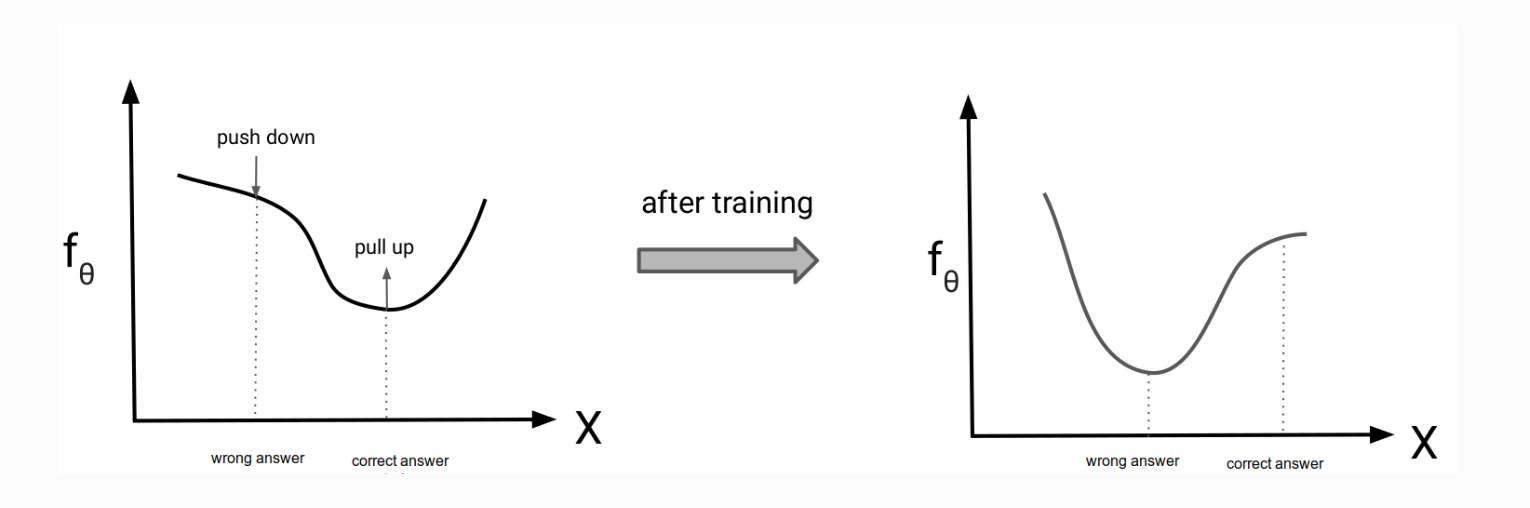
\includegraphics[width=1\textwidth]{figures/energy_based_model_contrastive_divergence_training}
    \caption{对比散度训练前后对比}\label{fig:energy_based_model_contrastive_divergence_training}
\end{figure}

式{\ref{eq:energy_based_model_nnl_contrastive_divergence}}中,
需要对概率分布{$q_{\theta}(\bm{x})$}采样。
可以应用朗志万动力学与马尔科夫链蒙特卡洛结合的方法采样,
即从随机数据点开始,
根据能量函数的梯度{$\nabla_{\bm{x}}E_{\theta}(\bm{x})$},使数据点的值向能量函数降低的方向移动。
此外,为避免陷入局部最小值,
需要在每一次更新梯度时添加噪声{$\omega \backsim \mathcal{N}(0,\sigma) $}。
理论上讲,根据梯度进行足够多次数据点取值更新,即可以准确地从概率分布{$q_{\theta}(\bm{x})$}采样,
但在实际中,通常将马尔科夫链的链长限制为{$K$},即进行{$K$}次取值更新。
算法{\ref{alg:energy_based_model_sampling}}为从基于能量的模型采样的算法。
\begin{algorithm}[ht]
    \caption{从基于能量的模型采样}\label{alg:energy_based_model_sampling}
    \begin{algorithmic}[1]
    \STATE{从高斯分布或均匀分布中采样{$\bm{\tilde{x}}^{0}$}}
    \FOR{采样步骤 {$k=1$}到 {$K$} }
    \STATE{{$\bm{\tilde{x}}^{k} \leftarrow \bm{\tilde{x}}^{k-1}- \eta\nabla_{\bm{x}}E_{\theta}(\bm{\tilde{x}}^{k-1}) + \omega  $},其中{$\omega \sim \mathcal{N}(0,\sigma)$}}
    \ENDFOR
    \STATE{$\bm{x}_{sample} \leftarrow \bm{\tilde{x}}^{K}$}
    \end{algorithmic}
\end{algorithm}



\subsubsection{变分自编码器}

自编码器是一个包含了两部分的神经网络,
其编码器可以将原始高维输入映射到低维隐变量空间,
解码器可以将隐变量空间中的低维表示恢复成原始输入{\cite{weng2018VAE}}。
通过使用自编码器,可以对数据进行更高效地压缩。
\begin{figure}[ht]
    \centering
    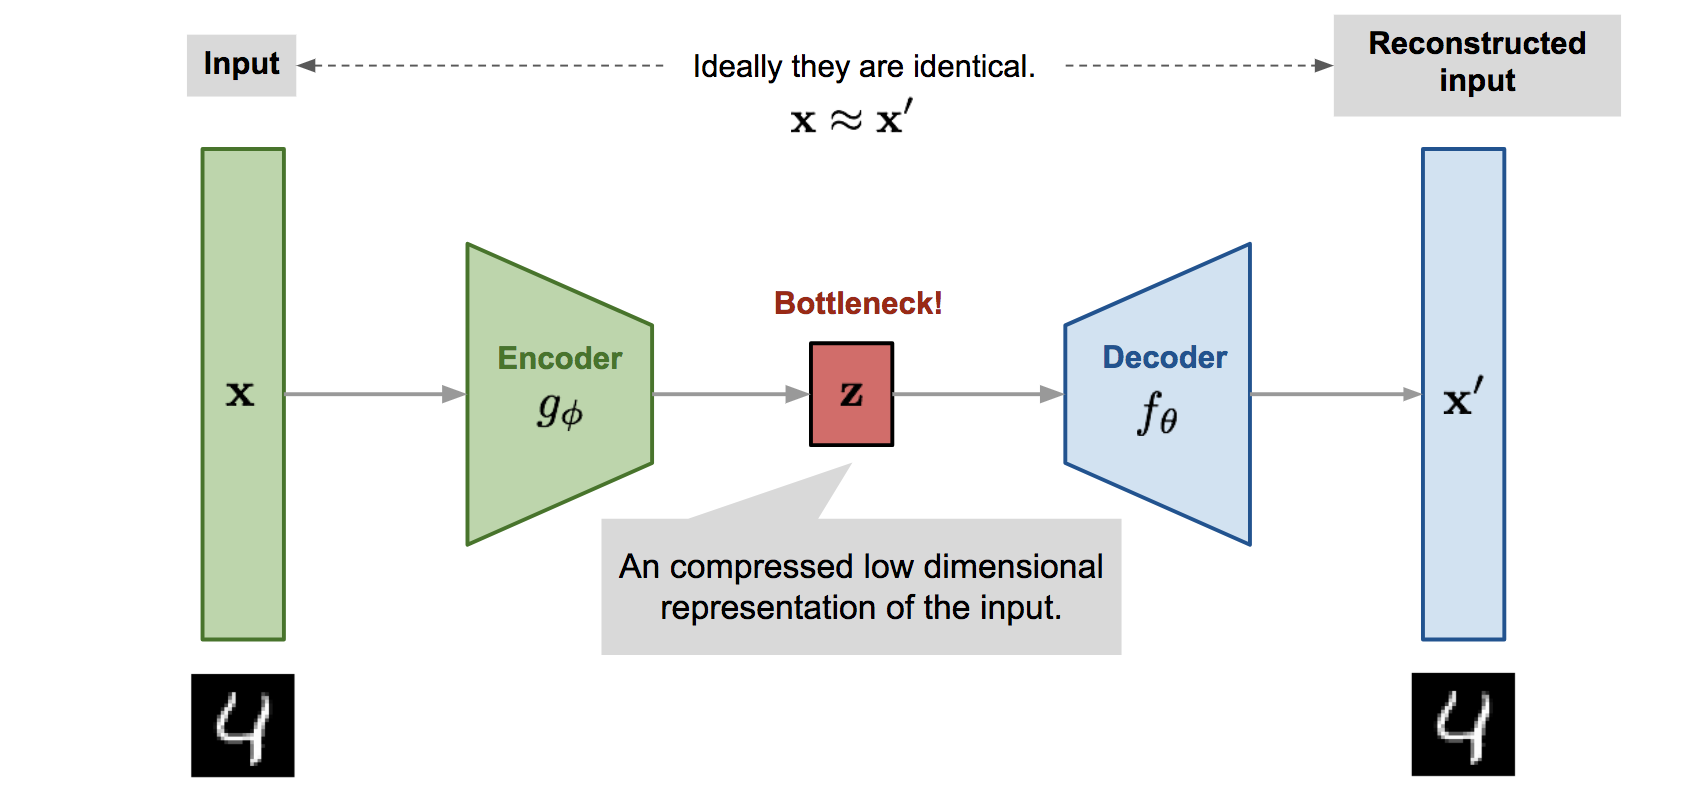
\includegraphics[width=1\textwidth]{figures/autoencoder}
    \caption{自编码器示意图}\label{fig:autoencoder}
\end{figure}

图{\ref{fig:autoencoder}}中,
{$\bm{x}$}表示样本,
{$\bm{x}^{'}$}表示对原始样本的重构,
{$\bm{z}$}表示样本在隐变量空间的表示,
{$g_{\phi}(.)$}表示由参数{$\phi$}确定的编码器函数,
{$f_{\theta}(.)$}表示由参数{$\theta$}确定的解码器函数。
\begin{equation}
    \label{eq:vae_encoder}
    \bm{z}=g_{\phi}(\bm{x})
\end{equation}
\begin{equation}
    \label{eq:vae_decoder}
    \bm{x}^{'}=f_{\theta}(g_{\phi}(\bm{x}))
\end{equation}

参数{$(\theta,\phi)$}可以通过比较原始样本值{$\bm{x}$}与重构样本值{$\bm{x}^{'}$}来学习,
如使用均方误差:
\begin{equation}
    \label{eq:autoencoder_loss}
    L_{AE}(\theta,\phi)=\frac{1}{n} \sum_{i=1}^{n}(\bm{x}^{(i)} - f_{\theta}(g_{\phi}(\bm{x})))
\end{equation}

为避免过拟合,
降噪自编码器{ {\cite{vincent2008extracting}}}对原始样本添加随机噪声:
\begin{align}
    \hat{\bm{x}}^{(i)} 
    & \backsim \mathcal{M}_{\mathcal{D}}(\hat{\bm{x}}^{(i)} \mid \bm{x}^{(i)}) \label{eq:denoising_autoencoder_corrupt}   \\
    L_{DAE}(\theta,\phi)
    &=\frac{1}{n} \sum_{i=1}^{n}(\bm{x}^{(i)} - f_{\theta}(g_{\phi}(\hat{\bm{x}}^{(i)} ))) \label{eq:denoising_autoencoder_loss}
\end{align}

式{\ref{eq:denoising_autoencoder_corrupt}}中,
{$\hat{\bm{x}}^{(i)} $}表示对原始样本值{$\bm{x}$}添加随机噪声或者进行掩码处理后的值,
{$\mathcal{D}$}为原始样本所在数据集,
{$ \mathcal{M}_{\mathcal{D}}$}表示从原始样本到{$\hat{\bm{x}}^{(i)} $}的映射。
式{\ref{eq:denoising_autoencoder_loss}}与式{\ref{eq:autoencoder_loss}}相比,
不再将重构样本与原始样本{$\bm{x}$}进行比较,
而是与添加随机噪声或进行掩码处理后的{$\hat{\bm{x}}^{(i)} $}进行比较。
图{\ref{fig:denoising_autoencoder_architecture}}为降噪自编码器结构图。
\begin{figure}[ht]
    \centering
    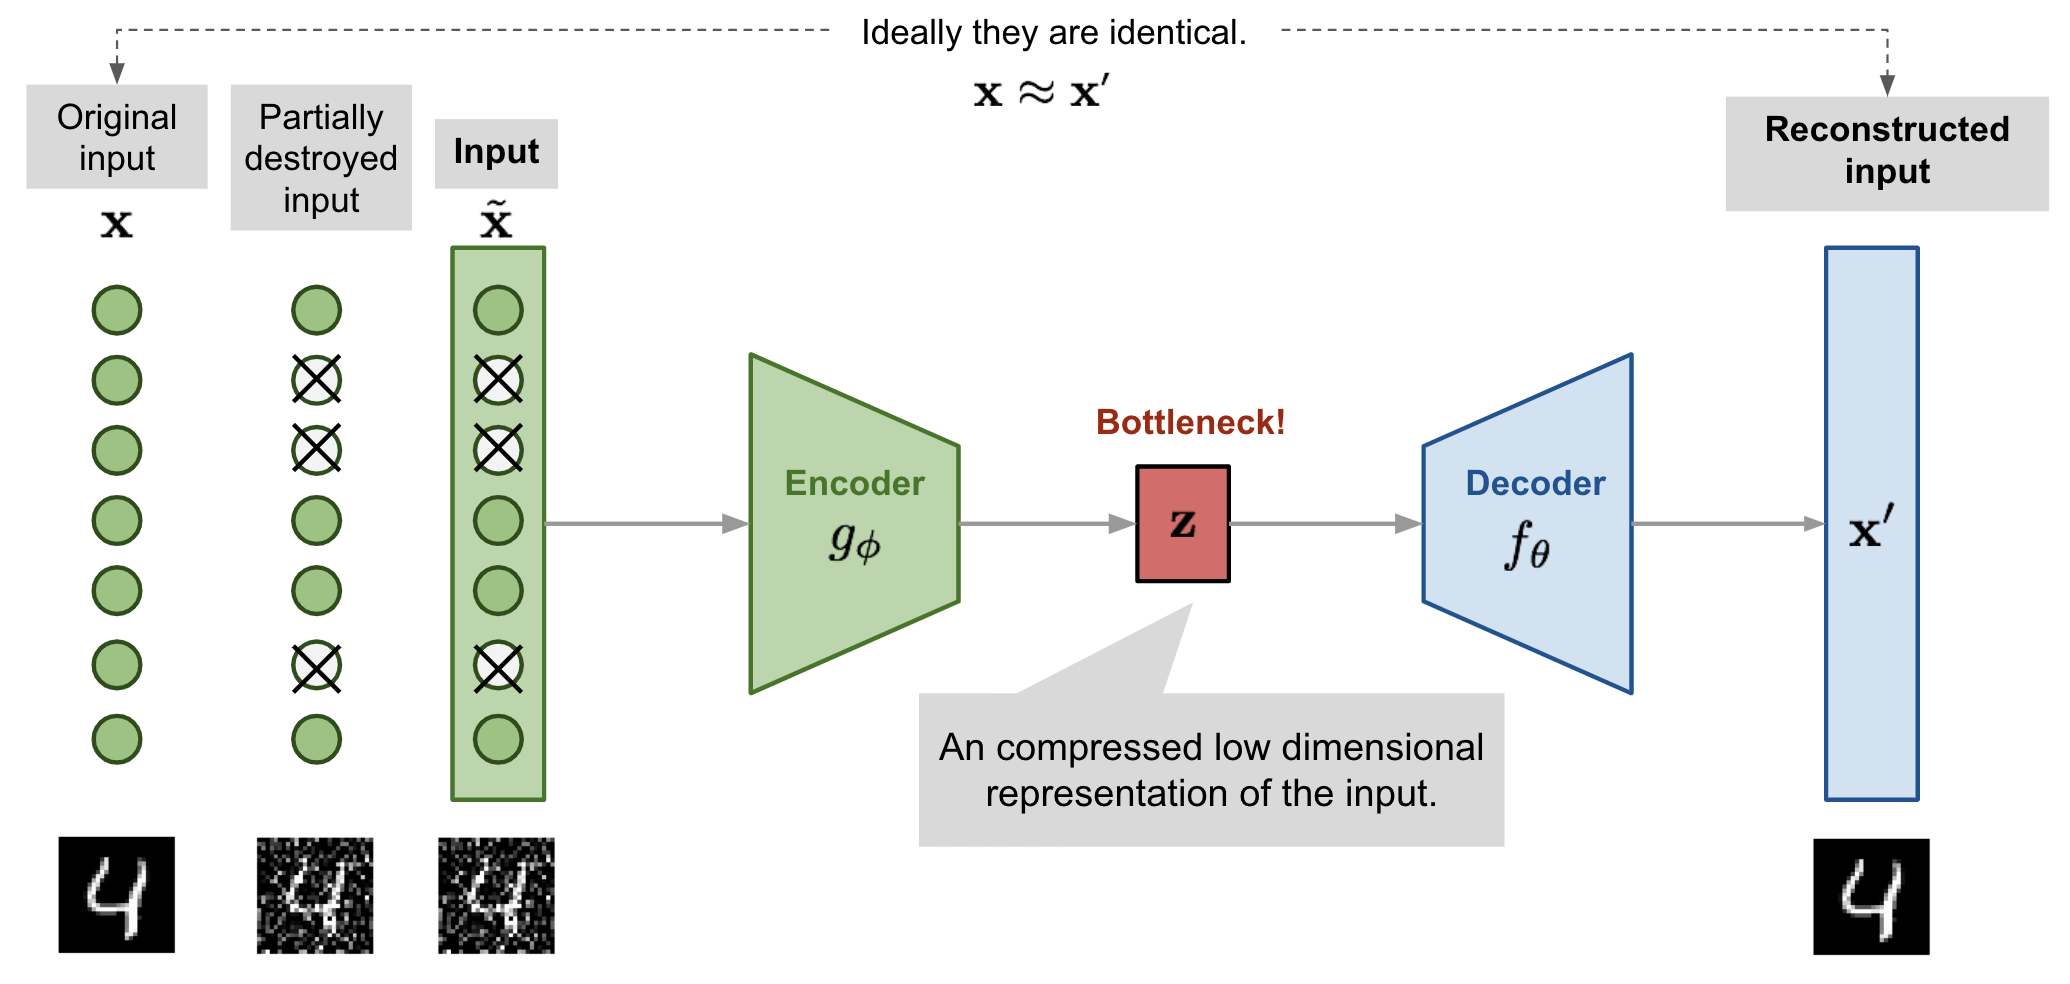
\includegraphics[width=1\textwidth]{figures/denoising_autoencoder_architecture}
    \caption{降噪自编码器结构}\label{fig:denoising_autoencoder_architecture}
\end{figure}

相比于自编码器和降噪自编码器,
变分自编码器并不将样本映射到一个固定的向量
而是映射到一个由参数{$\theta$}确定的概率分布{$p_{\theta}$}。
输入样本{$\bm{x}$}和隐变量{$\bm{z}$}的关系可以定义为:
\begin{itemize}
    \item 先验概率{$p_{\theta}(\bm{z})$};
    \item 似然函数{$p_{\theta}(\bm{x}\mid \bm{z})$};
    \item 后验概率{$p_{\theta}(\bm{z}\mid \bm{x})$}。
\end{itemize}

若知道概率分布{$p_{\theta}$}的真实参数值{$\theta ^{*}$},
则生成样本点某一维度的值{$\bm{x}^{(i)}$}(如图片样本的一个像素值)需要两个步骤:
\begin{enumerate}
    \item 从先验分布{$p_{\theta^{*}}(\bm{z})$}中采样获得{$\bm{z}^{(i)}$};
    \item 从条件概率{$p_{\theta^{*}}(\bm{x}\mid \bm{z}=\bm{z}^{(i)})$}中生成值{$\bm{x}^{(i)}$}。
\end{enumerate}

最优参数值{$\theta^{*}$}可以通过最大化生成真实数据样本的概率获得,即:
\begin{equation}
    \label{eq:vae_maximum_likelihood}
    \theta ^{*}=\argmax_{\theta}\prod_{i=1}^{n}p_{\theta}(\bm{x}^{(i)})
\end{equation}
取对数可得:
\begin{equation}
    \label{eq:vae_maximux_log_likelihood}
    \theta ^{*}=\argmax_{\theta}\sum_{i=1}^{n}\log p_{\theta}(\bm{x}^{(i)})
\end{equation}
式{\ref{eq:vae_maximux_log_likelihood}}中,
{$p_{\theta}(\bm{x}^{(i)})$}
可以表示为:
\begin{equation}
    \label{eq:var_probability_of_xi}
    p_{\theta}(\bm{x}^{(i)})=\int p_{\theta}(\bm{x}^{(i)} \mid \bm{z}) p_{\theta}(\bm{z}) d\,{\bm{z}}
\end{equation}

但由于某些隐变量无法积分或计算开销巨大,
式{\ref{eq:var_probability_of_xi}}无法直接计算。
可用证据下界式{\ref{eq:evidence_lower_bound}}来近似对数似然函数。
使用证据下界可以获得对后验概率{$p_{\theta}(\bm{z}\mid\bm{x})$}的近似,
即由参数{$\phi$}确定的{$q_{\phi}(\bm{z}\mid\bm{x})$}。
图{\ref{fig:vae_elbo}}中,
近似函数{$q_{\phi}(\bm{z}\mid\bm{x})$}定义了编码器,
条件概率{$p_{\theta}(\bm{x}\mid\bm{z})$}定义了解码器。
\begin{figure}[ht]
    \centering
    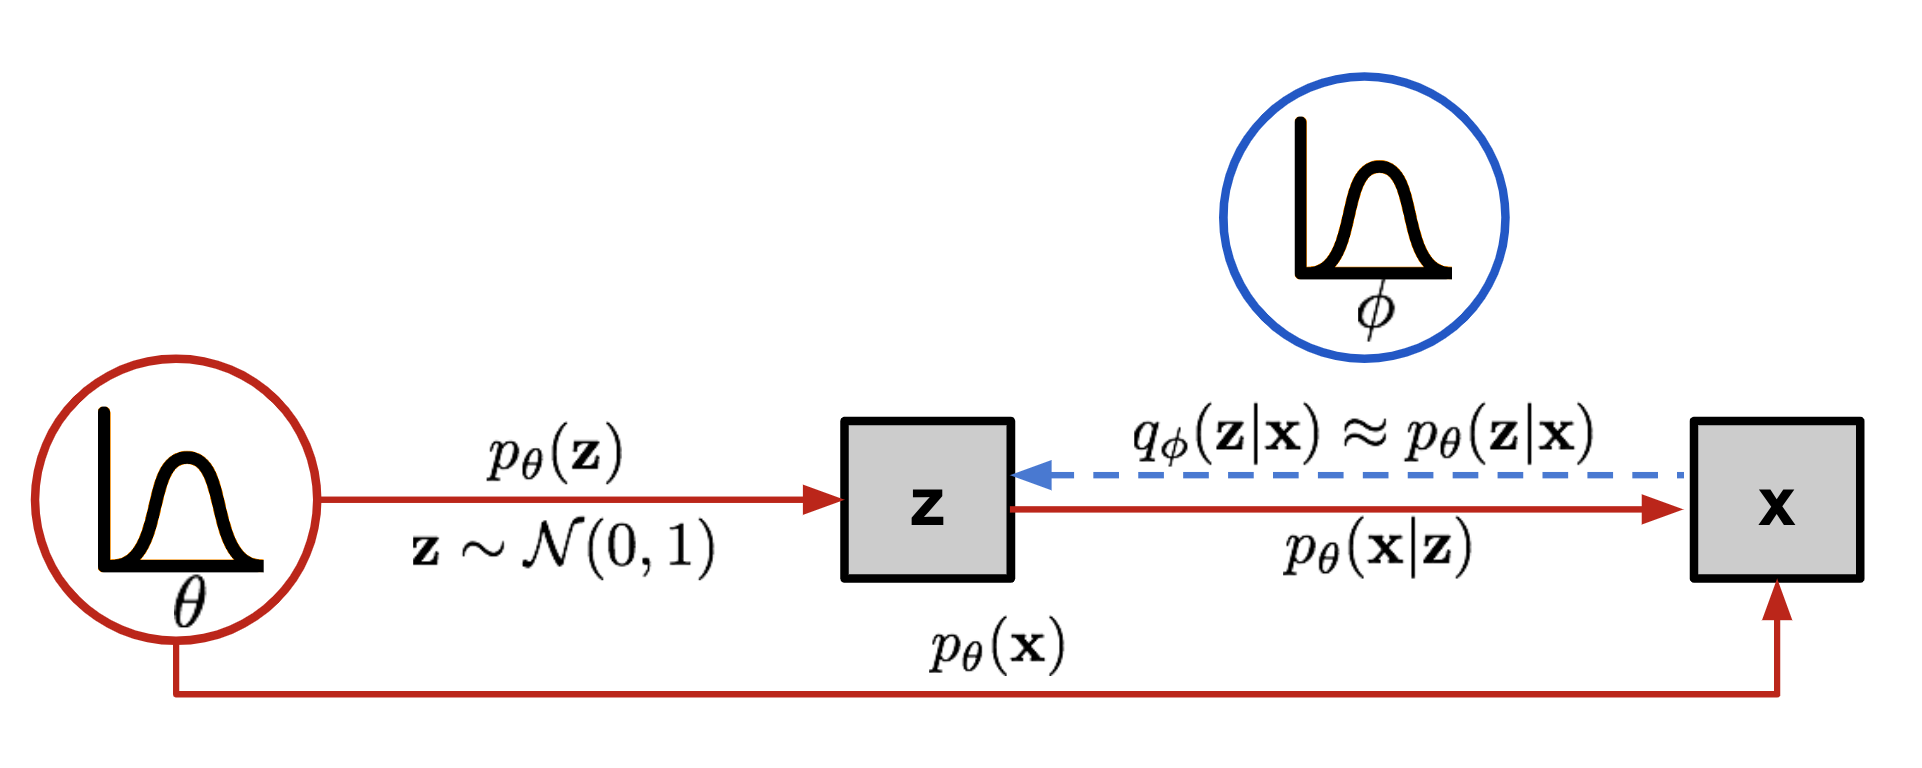
\includegraphics[width=\textwidth]{figures/vae_elbo}
    \caption{使用ELBO近似变分自编码器对数似然函数}\label{fig:vae_elbo}
\end{figure}

对证据下界式{\ref{eq:evidence_lower_bound}}变形可得:
\begin{align}
    \mathbb{E}_{q_{\phi}(\bm{z}|\bm{x})}\left[\log\frac{p(\bm{x},\bm{z})}{q_{\phi}(\bm{z}\mid\bm{x})}\right]
    &=\mathbb{E}_{q_{\phi}(\bm{z}|\bm{x})}\left[\log\frac{p_{\theta}(\bm{x}\mid \bm{z})p(\bm{z})}{q_{\phi}(\bm{z}\mid\bm{x})}\right] \\
    &=\mathbb{E}_{q_{\phi}(\bm{z}|\bm{x})}\left[\log p_{\theta}(\bm{x}\mid \bm{z})\right] + \mathbb{E}_{q_{\phi}(\bm{z}|\bm{x})}\left[\log\frac{p(\bm{z})}{q_{\phi}(\bm{z}\mid\bm{x})}\right]\\
    &=\underbrace{\mathbb{E}_{q_{\phi}(\bm{z}|\bm{x})}\left[\log p_{\theta}(\bm{x}\mid \bm{z})\right] }_{\mbox{重构项}} -\underbrace{ D_{KL}(q_{\phi}(\bm{z}\mid \bm{x}) \mid \mid p(\bm{z}))}_{\mbox{先验匹配项}}  \label{eq:vae_elbo_dissect}
\end{align}

式{\ref{eq:vae_elbo_dissect}}中,
重构项度量了解码器相对于变分分布{$q_{\phi}(\bm{z}\mid \bm{x})$}的重构似然函数{$p_{\theta}(\bm{x}\mid \bm{z})$},
从而使学到的分布可以对隐变量有效地建模,以便于可以通过{$p_{\theta}(\bm{x}\mid\bm{z})$}进行原样本重构。
先验匹配项度量了学到的变分分布与隐变量先验分布的相似度,
从而保证编码器能够真正学到隐变量分布而不是记忆原样本到隐变量的映射。
最大化证据下界等价于最大化重构项和最小化先验匹配项。
\begin{figure}[ht]
    \centering
    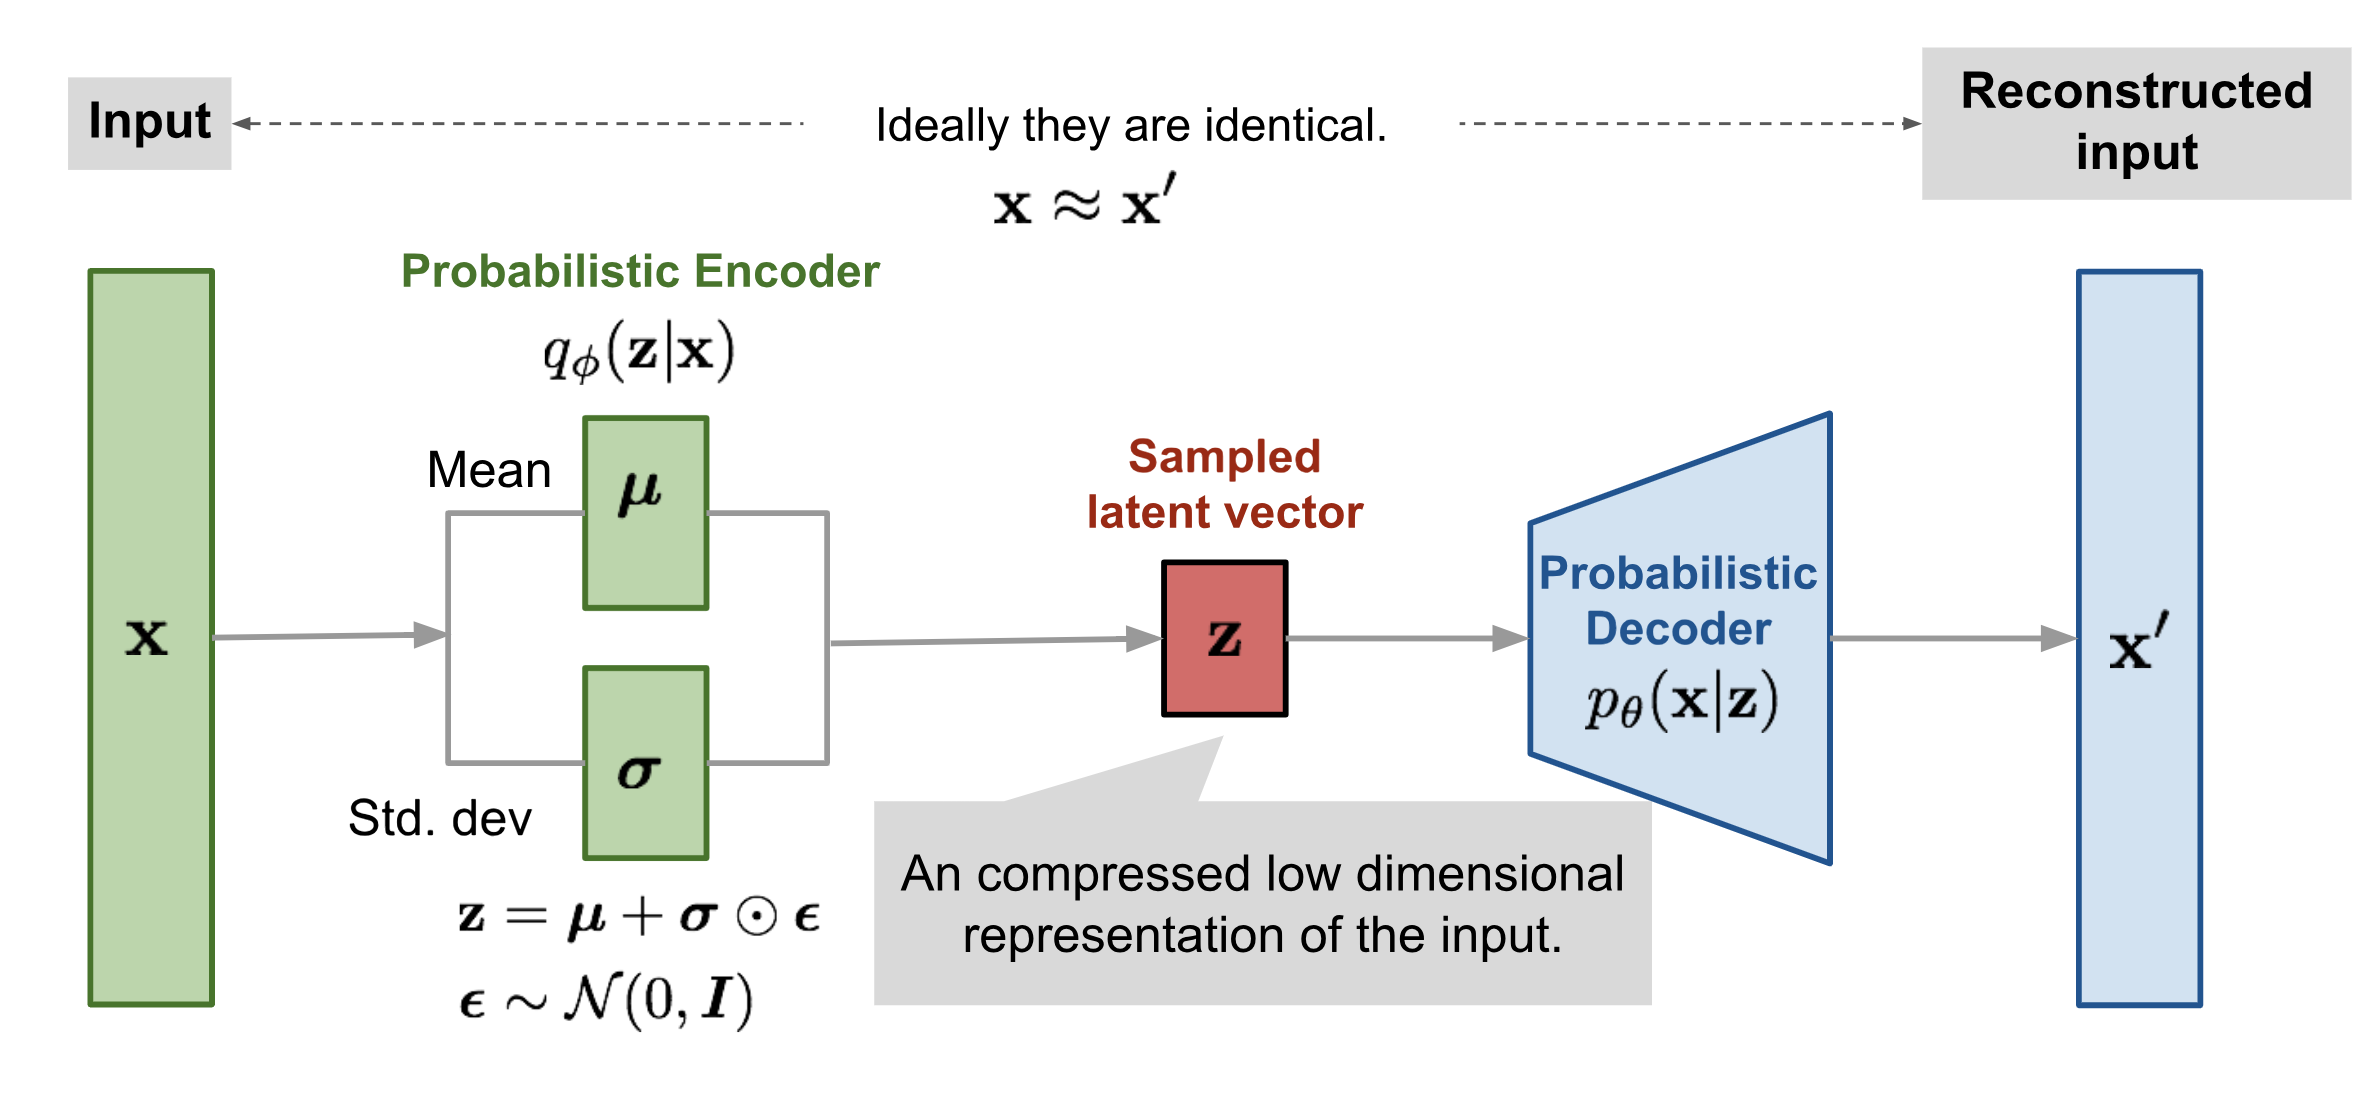
\includegraphics[height=0.4\textwidth]{figures/vae}
    \caption{变分自编码器}\label{fig:vae}
\end{figure}


变分自编码器中,通常编码器都为具有对角协方差矩阵的多变量高斯分布,隐变量的先验分布为多变量标准高斯分布:
\begin{equation}
    \label{eq:vae_q_phi_z_mid_x_gaussian}
    q_{\phi}(\bm{z}\mid\bm{x})=\mathcal{N}(\bm{z};\bm{\mu}_{\phi}(\bm{x},\bm{\sigma}_{\phi}^{2}(\bm{x})\bm{I}))
\end{equation}
\begin{equation}
    \label{eq:vae_p_z_gaussian}
    p(\bm{z})=\mathcal{N}(\bm{z};\bm{0},\bm{I})
\end{equation}

因此,
由式{\ref{eq:vae_q_phi_z_mid_x_gaussian}}和式{\ref{eq:vae_p_z_gaussian}}可以计算式{\ref{eq:vae_elbo_dissect}}中的先验匹配项。
而式{\ref{eq:vae_elbo_dissect}}中的重构项可以由蒙特卡洛方法进行估计,
即:
\begin{align}
   &\argmax_{\phi,\theta} \mathbb{E}_{q_{\phi}(\bm{z}|\bm{x})}\left[\log p_{\theta}(\bm{x}\mid \bm{z})\right]  - D_{KL}(q_{\phi}(\bm{z}\mid \bm{x}) \mid \mid p(\bm{z})) \label{eq:vae_argmax-elbo} \\
   &\approx  \argmax_{\phi,\theta} \sum_{l=1}^{L} \log p_{\theta}(\bm{x}\mid \bm{z}^{(l)}) - D_{KL}(q_{\phi}(\bm{z}\mid \bm{x}) \mid \mid p(\bm{z}))  \label{eq:vae_max_elbo_approx}
\end{align}
式{\ref{eq:vae_max_elbo_approx}}中,{${\bm{z}^{(l)}}_{l=1}^{L}$}为关于数据集中每个样本{$\bm{x}$}从{$q_{\phi}(\bm{z}\mid\bm{x})$}中获得的采样。

但由于通过随机过程获得的采样{$\bm{z}^{(l)}$}不可微,
无法计算梯度,
根据重参数方法式{\ref{eq:reparameterization_trick}}可得:
\begin{equation}
    \label{eq:vae_reparameterization_trick}
    \bm{z}=\bm{\mu}_{\phi}{(\bm{x})}+\bm{\sigma}_{\phi}(\bm{x})\odot \bm{\epsilon} \mbox{\qquad 其中 }\epsilon \sim \mathcal{N}(\bm{\epsilon};\bm{0},\bm{I})
\end{equation}

式{\ref{eq:vae_reparameterization_trick}}中,
{$\odot$}为对应元素分别相乘。
图{\ref{fig:vae_reparameterization_trick}}中,重参数方法使损失梯度不可反向传播的过程变为可以反向传播。
\begin{figure}[ht]
    \centering
    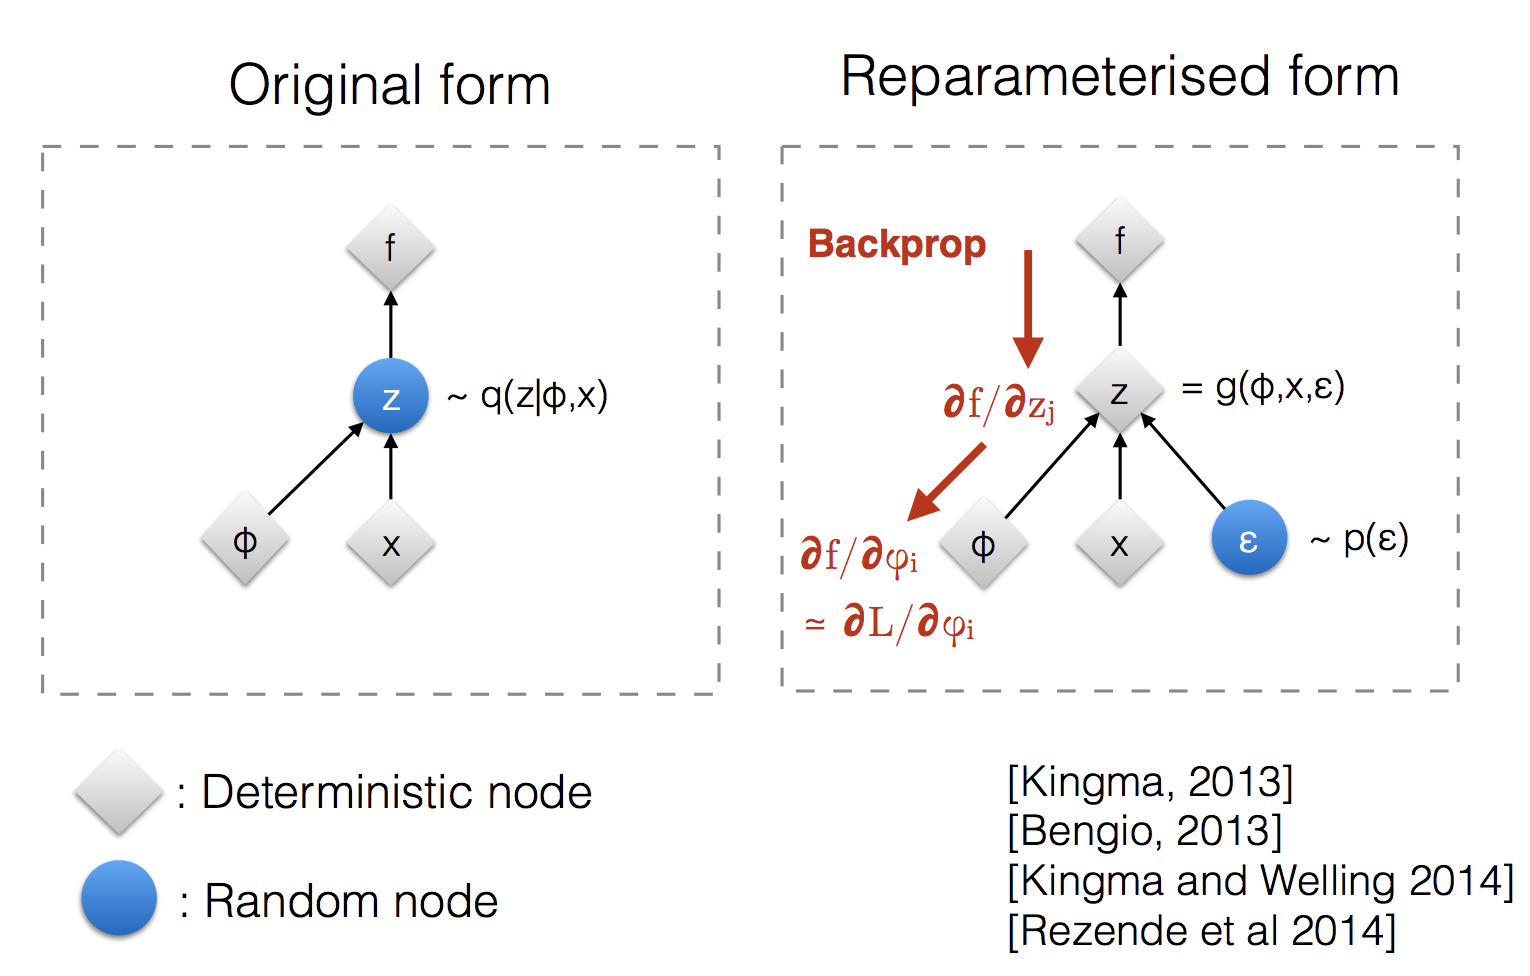
\includegraphics[height=0.45\textwidth]{figures/vae_reparameterization_trick}
    \caption{重参数方法示意图}\label{fig:vae_reparameterization_trick}
\end{figure}

式{\ref{eq:vae_max_elbo_approx}}中,变分自编码器使用重参数方法和蒙特卡洛方法,
对证据下界关于{$\phi$}和{$\theta$}同时进行优化。
训练完成后,即可直接从隐变量分布{$p(\bm{z})$}中进行采样,再经由解码器获得生成样本{$\bm{x}'$}。

层级变分自编码器是对变分自编码器的扩展{\cite{Luo2022UnderstandingDM}},
相比于变分自编码器,
层级变分自编码器可以有多层隐变量。
层级变分自编码器假设浅层隐变量由更深层的隐变量生成。
对于有{$T$}层隐变量的层级变分自编码器,
每一个隐变量都依赖于先前所有隐变量,
而其一个特例为马尔可夫层级变分自编码器。
马尔可夫层级变分自编码器中,
生成过程为马尔可夫链,
解码时每一个隐变量{$\bm{z}_{t}$}只依赖于之前一个隐变量{$\bm{z}_{t+1}$},
图{\ref{fig:markovian_hierarchical_variational_autoencoder}}为马尔可夫层级变分自编码器示意图。
\begin{figure}[ht]
    \centering
    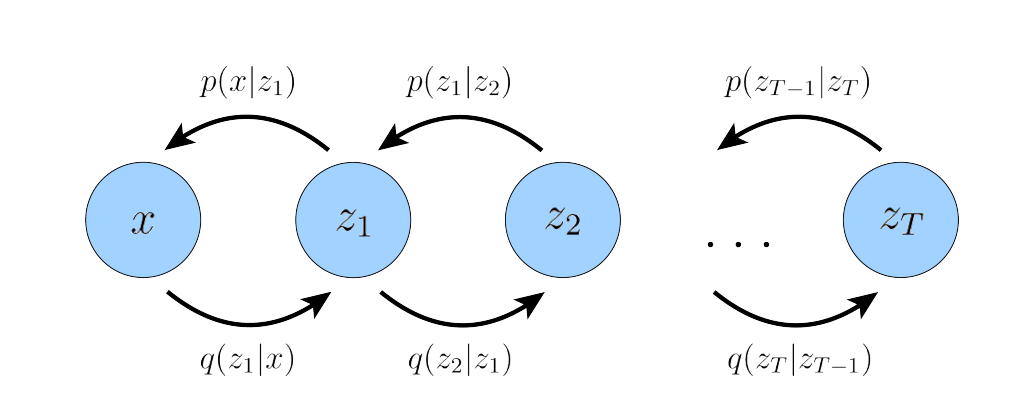
\includegraphics[width=0.8\textwidth]{figures/markovian_hierarchical_variational_autoencoder}
    \caption{马尔可夫层级变分自编码器示意图}\label{fig:markovian_hierarchical_variational_autoencoder}
\end{figure}

马尔可夫层级变分自编码器的联合概率分布可以表示为:
\begin{equation}
    \label{eq:mhvae_joint_distribution}
    p(\bm{x},\bm{z}_{1:T})=p(\bm{x}_{T})p_{\theta}(\bm{x}\mid \bm{z}_{1})\prod_{t=2}^{T}p_{\theta}(\bm{z}_{t-1}\mid\bm{z}_{t})
\end{equation}
其后验概率可以表为:
\begin{equation}
    \label{eq:mhvae_posterior}
    q_{\phi}(\bm{z}_{1:T} \mid \bm{x})=q_{\phi}(\bm{z}_{1}\mid \bm{x})\prod_{t=2}^{T}q_{\phi}(\bm{z}_{t}\mid\bm{z}_{t-1})
\end{equation}
证据下界可以扩展为:
\begin{align}
    \log p(\bm{x})
    & =\log \int p(\bm{x},\bm{z}_{1:T}) d\,z & \mbox{(根据式{\ref{eq:elbo_probability_of_x_with_integral}})} \\
    &=\log \int p(\bm{x},\bm{z}_{1:T})  \frac{q_{\phi}(\bm{z}_{1:T}\mid\bm{x})}{q_{\phi}(\bm{z}_{1:T}\mid\bm{x})} d\,z \\
    &=\log \int \frac{p(\bm{x},\bm{z}_{1:T}) q_{\phi}(\bm{z}_{1:T}\mid\bm{x})}{q_{\phi}(\bm{z}_{1:T}\mid\bm{x})} d\,z \\
    &=\log \int q_{\phi}(\bm{z}_{1:T}\mid\bm{x}) \frac{p(\bm{x},\bm{z}_{1:T}) }{q_{\phi}(\bm{z}_{1:T}\mid\bm{x})} d\,z \\
    &= \log \mathbb{E}_{q_{\phi}(\bm{z}_{1:T}|\bm{x})}\left[\frac{p(\bm{x},\bm{z}_{1:T})}{q_{\phi}(\bm{z}_{1:T}\mid\bm{x})}\right]  & \mbox{(根据期望定义式{\ref{eq:expection_continuous}})} \\
    &\geq \mathbb{E}_{q_{\phi}(\bm{z}_{1:T}|\bm{x})}\left[\log\frac{p(\bm{x},\bm{z}_{1:T})}{q_{\phi}(\bm{z}_{1:T}\mid\bm{x})}\right] & \mbox{(根据杰森不等式{\ref{eq:Jensen_ineuqality}})} \label{eq:mhvae_elbo_jensen_inequaality}
\end{align}
将式{\ref{eq:mhvae_joint_distribution}}与{\ref{eq:mhvae_posterior}}代入式{\ref{eq:mhvae_elbo_jensen_inequaality}}可得:
\begin{equation}
\label{eq:mhvae_elbo_with_substitution}
\mathbb{E}_{q_{\phi}(\bm{z}_{1:T}|\bm{x})}\left[\log\frac{p(\bm{x},\bm{z}_{1:T})}{q_{\phi}(\bm{z}_{1:T}\mid\bm{x})}\right] 
=\mathbb{E}_{q_{\phi}(\bm{z}_{1:T}|\bm{x})}\left[\log\frac
{p(\bm{z}_{T})p_{\theta}(\bm{x}\mid \bm{z}_{1})\prod_{t=2}^{T}p_{\theta}(\bm{z}_{t-1}\mid\bm{z}_{t})}
{q_{\phi}(\bm{z}_{1}\mid \bm{x})\prod_{t=2}^{T}q_{\phi}(\bm{z}_{t}\mid\bm{z}_{t-1})}
\right] 
\end{equation}

在扩散模型中,
式{\ref{eq:mhvae_elbo_with_substitution}}可以进一步分解更具有意义的成分。

此外,由于自编码器与降噪自编码器并不直接定义似然函数,
可以将自编码器和降噪自编码器视为隐式密度模型。
而变分自编码器由于使用证据下界对似然函数进行近似,
变分自编码器为近似估计的显示密度模型。



\subsubsection{扩散模型}
% 扩散模型历史
% 扩散模型结构
扩散模型,是近年来在生成图像领域最有影响力的模型之一。
在很多评价基准上,扩散模型已经取得了相比生成对抗网络更好的成绩。
就如2017——2020年生成对抗网络的流行,在2022年,扩散模型也被广泛地用于各项生成任务。

2015年,扩散模型被从物理学中借鉴引入至深度学习领域 {\cite{sohl2015deep}}。
2019年,基于分数的模型NCSN {\cite{song2019generative}}的提出,
以及2020年对基于分数的模型训练方法的改进,都为扩散模型的诞生打下了良好的基础。

扩散模型可以理解为加一定限制的马尔可夫层级变分自编码器:
\begin{enumerate}
    \item 隐变量维度与样本维度相同;
    \item 每一时间(层级)隐变量编码器的结构为预先定义的线性高斯模型,并非学习获得,即将前一层隐变量值作为高斯分布的均值;
    \item 隐变量编码器高斯分布的参数随着时间(层级)的变化而变化,且保证最终的隐变量分布为标准高斯分布。
\end{enumerate}
\begin{figure}[ht]
    \centering
    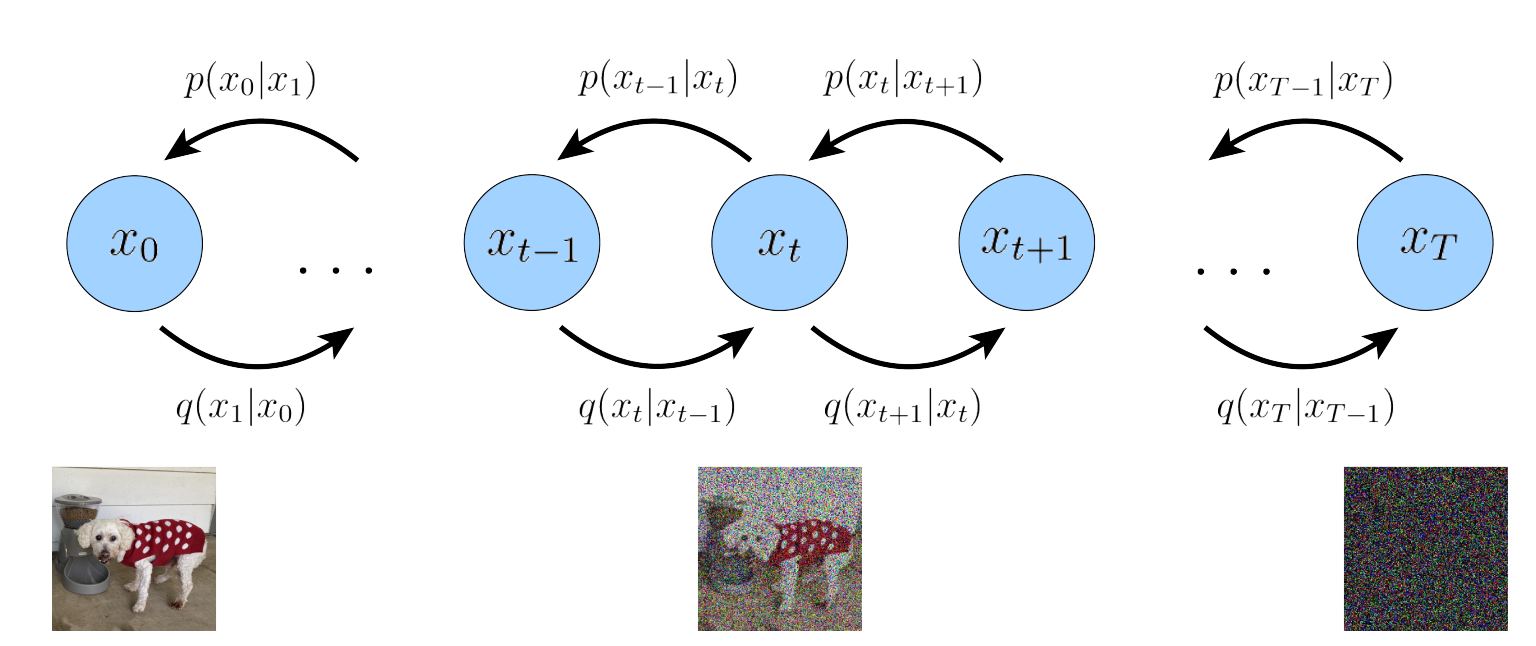
\includegraphics[width=\textwidth]{figures/diffusion_model}
    \caption{扩散模型示意图}\label{fig:diffusion_model}
\end{figure}

图{\ref{fig:diffusion_model}}为扩散模型示意图,
{$\bm{x}_{0}$}表示真实样本,如自然图像,
{$\bm{x}_{T}$}表示完全的高斯噪声,
{$\bm{x}_{t}$}表示真实样本{$\bm{x}_{0}$}添加噪声后所得的隐变量。
{$q(\bm{x}_{t}\mid \bm{x}_{t-1})$}为将前一状态作为均值的高斯分布。

由第一个假设,将真实样本和隐变量均由{$\bm{x}_{t}$}表示,
其中{$t=0$}表示真实样本,
{$t\in \left[1,T \right]$}表示相应的{$t$}层隐变量,
则扩散模型的后验与马尔可夫层级变分自编码器相似,
根据式{\ref{eq:mhvae_posterior}}得:
\begin{equation}
    \label{eq:diffusion_posterior}
    q(\bm{x}_{1:T} \mid \bm{x}_{0})=\prod_{t=1}^{T}q(\bm{x}_{t}\mid\bm{x}_{t-1})
\end{equation}

由第二个假设,编码器中隐变量服从以前一隐变量为均值的高斯分布,
与马尔可夫结构变分自编码器不同的是,
编码器在每一时间步{$t$}的结构并非学习获得,
而是预先设定的线性高斯模型,
均值和方差可以设为超参数{ {\cite{ho2020denoising}}},
或经学习获得{ {\cite{kingma2023variational}}}。
设高斯编码器均值为{$\bm{\mu}_{t}(\bm{x}_{t})=\sqrt{a_{t}}\bm{x}_{t-1}$},
方差为{$\bm{\Sigma}_{t}(\bm{x}_{t}) = (1-\alpha_t)\bm{I}$},
以使隐变量的方差大小相近。
为使模型更灵活,{$\alpha_t$}的值可以随着层级深度{$t$}的变化而变化。
编码转换过程可以表示为:
\begin{equation}
    \label{eq:diffusion_encoder}
    q(\bm{x}_{t}\mid \bm{x}_{t-1})=\mathcal{N}(\bm{x}_{t}; \sqrt{\alpha}_{t}(\bm{x}_{t-1}), (1-\alpha_t)\bm{I})
\end{equation}

由第三个假设,
预先定义或可学习获得的{$\alpha_t$}可以随着时间的变换而变化,
且最深层隐变量{$p(\bm{x}_T)$}的分布为标准高斯分布,
则马尔可夫层级变分自编码器的联合概率分布式{\ref{eq:mhvae_joint_distribution}}可以改写为:
\begin{equation}
    \label{eq:diffusion_joint_distribution}
    p(\bm{x}_{0:T})=p(\bm{x}_{T})\prod_{t=1}^{T}p_{\theta}(\bm{x}_{t-1}\mid\bm{x}_{t})
\end{equation}
式{\ref{eq:diffusion_joint_distribution}}中,
{$p(\bm{x}_T) = \mathcal{N}(\bm{x}_{T};\bm{0},\bm{I})$}。
假设三表明,扩散模型逐渐向图片添加噪声直至图片变为完全的高斯噪声,即如图{\ref{fig:diffusion_model}}所示。

相比于马尔可夫层级变分自编码器,
编码器分布{$q(\bm{x}_t\mid \bm{x}_{t-1})$}不再由参数{$\phi$}定义,
而完全服从预先定义了均值与方差的高斯分布。
因此,为能够生成新的样本点,
扩散模型更注重对条件概率{$p_{\theta}(\bm{x}_{t-1}\mid \bm{x}_{t})$}的学习。
对扩散模型优化后,
采样过程即为首先从高斯噪声{$p(\bm{x}_T)$}中采样,
随后连续地进行{$T$}次去噪变换{$p_{\theta}(\bm{x}_{t-1}\mid \bm{x}_{t})$},
最终获得新的样本点{$\bm{x}_{0}$}。

类比于层级变分自编码器,扩散模型可以通过最大化证据下界来优化,即:
\begin{align}
    \log p(\bm{x})
    &= \log \int p(\bm{x}_{0:T}) d\, \bm{x}_{1:T}
    \\ & = \log \int p(\bm{x}_{0:T}) \frac{q(\bm{x}_{1:T}\mid \bm{x}_{0})}{q(\bm{x}_{1:T}\mid \bm{x}_{0})} d\, \bm{x}_{1:T}
    \\ & = \log \int q(\bm{x}_{1:T}\mid \bm{x}_{0}) \frac{p(\bm{x}_{0:T}) }{q(\bm{x}_{1:T}\mid \bm{x}_{0})} d\, \bm{x}_{1:T}
    \\ & = \log \mathbb{E}_{q(\bm{x}_{1:T}\mid \bm{x}_{0})} \left[     \frac{p(\bm{x}_{0:T}) }{q(\bm{x}_{1:T}\mid \bm{x}_{0})}     \right]
    \\ & \geq  \mathbb{E}_{q(\bm{x}_{1:T}\mid \bm{x}_{0})} \left[   \log  \frac{p(\bm{x}_{0:T}) }{q(\bm{x}_{1:T}\mid \bm{x}_{0})}     \right] \label{eq:diffusion_elbo_origin}
    \\ & = \mathbb{E}_{q(\bm{x}_{1:T}\mid \bm{x}_{0})} \left[   \log  \frac{p(\bm{x}_{T}) \prod_{t=1}^{T}{p_{\theta}(\bm{x}_{t-1}\mid \bm{x}_{t})} }{\prod_{t=1}^{T}{q(\bm{x}_{t}\mid \bm{x}_{t-1})} }     \right]
    \\ & = \mathbb{E}_{q(\bm{x}_{1:T}\mid \bm{x}_{0})} \left[   \log  \frac{p(\bm{x}_{T})p_{\theta}(\bm{x}_{0} \mid \bm{x}_1) \prod_{t=2}^{T}{p_{\theta}(\bm{x}_{t-1}\mid \bm{x}_{t})} }{q(\bm{x}_{T}\mid \bm{x}_{T-1})\prod_{t=1}^{T-1}{q(\bm{x}_{t}\mid \bm{x}_{t-1})} }     \right]
    \\ & = \mathbb{E}_{q(\bm{x}_{1:T}\mid \bm{x}_{0})} \left[   \log  \frac{p(\bm{x}_{T})p_{\theta}(\bm{x}_{0} \mid \bm{x}_1) \prod_{t=1}^{T-1}{p_{\theta}(\bm{x}_{t}\mid \bm{x}_{t+1})} }{q(\bm{x}_{T}\mid \bm{x}_{T-1})\prod_{t=1}^{T-1}{q(\bm{x}_{t}\mid \bm{x}_{t-1})} }     \right]
    \\ & = \mathbb{E}_{q(\bm{x}_{1:T}\mid \bm{x}_{0})} \left[   \log  \frac{p(\bm{x}_{T})p_{\theta}(\bm{x}_{0} \mid \bm{x}_1)  }{q(\bm{x}_{T}\mid \bm{x}_{T-1})}     \right]
    + \mathbb{E}_{q(\bm{x}_{1:T}\mid \bm{x}_{0})} \left[   \log \prod_{t=1}^{T-1} {\frac{p_{\theta}(\bm{x}_{t}\mid \bm{x}_{t+1})} {q(\bm{x}_{t}\mid \bm{x}_{t-1})} }     \right]
    \\ & = \mathbb{E}_{q(\bm{x}_{1:T}\mid \bm{x}_{0})} \left[   \log  p(\bm{x}_{T})\right]
    + \mathbb{E}_{q(\bm{x}_{1:T}\mid \bm{x}_{0})} \left[   \log  \frac{p_{\theta}(\bm{x}_{0} \mid \bm{x}_1)  }{q(\bm{x}_{T}\mid \bm{x}_{T-1})}     \right]
    \nonumber \\ &\qquad+ \mathbb{E}_{q(\bm{x}_{1:T}\mid \bm{x}_{0})} \left[   \sum_{t=1}^{T-1} { \log \frac{p_{\theta}(\bm{x}_{t}\mid \bm{x}_{t+1})} {q(\bm{x}_{t}\mid \bm{x}_{t-1})} }     \right]
    \\ & = \mathbb{E}_{q(\bm{x}_{1:T}\mid \bm{x}_{0})} \left[   \log  p(\bm{x}_{T})\right]
    + \mathbb{E}_{q(\bm{x}_{1:T}\mid \bm{x}_{0})} \left[   \log  \frac{p_{\theta}(\bm{x}_{0} \mid \bm{x}_1)  }{q(\bm{x}_{T}\mid \bm{x}_{T-1})}     \right]
    \nonumber \\ &\qquad+ \sum_{t=1}^{T-1} \mathbb{E}_{q(\bm{x}_{1:T}\mid \bm{x}_{0})} \left[    { \log \frac{p_{\theta}(\bm{x}_{t}\mid \bm{x}_{t+1})} {q(\bm{x}_{t}\mid \bm{x}_{t-1})} }     \right]
    \\ & = \mathbb{E}_{q(\bm{x}_{1}\mid \bm{x}_{0})} \left[  \log  p_{\theta}(\bm{x}_{0}\mid \bm{x}_{1})\right]
    + \mathbb{E}_{q(\bm{x}_{T-1},\bm{x}_{T}\mid \bm{x}_{0})} \left[   \log  \frac{p_{\theta}(\bm{x}_{0} \mid \bm{x}_1)  }{q(\bm{x}_{T}\mid \bm{x}_{T-1})}     \right]
    \nonumber \\ & \qquad+ \sum_{t=1}^{T-1} \mathbb{E}_{q(\bm{x}_{T-1},\bm{x}_{t},\bm{x}_{t+1}\mid \bm{x}_{0})} \left[    { \log \frac{p_{\theta}(\bm{x}_{t}\mid \bm{x}_{t+1})} {q(\bm{x}_{t}\mid \bm{x}_{t-1})} }     \right]
    \\ & = \underbrace{\mathbb{E}_{q(\bm{x}_{1}\mid \bm{x}_{0})} \left[   \log  p_{\theta}(\bm{x}_{0}\mid \bm{x}_{1})\right]}_{\mbox{重构项}}
    - \underbrace{\mathbb{E}_{q(\bm{x}_{T-1}\mid \bm{x}_{0})}{\left[D_{KL}(q(\bm{x}_{T}\mid \bm{x}_{T-1}) \Vert p(\bm{x}_{T}) )\right]}}_{\mbox{先验匹配项}}
    \nonumber \\ & \qquad - \sum_{t=1}^{T-1} \underbrace{\mathbb{E}_{q(\bm{x}_{t-1},\bm{x}_{t+1}\mid \bm{x}_0)} \left[ D_{KL}( q(\bm{x}_{t}\mid\bm{x}_{t-1} )  \Vert  p_{\theta}(\bm{x}_{t}\mid \bm{x}_{t+1})   )  \right]    }_{\mbox{一致检验项}} \label{eq:diffusion_elbo}
\end{align}
式{\ref{eq:diffusion_elbo}}中:
\begin{itemize}
    \item {$\mathbb{E}_{q(\bm{x}_{1}\mid \bm{x}_{0})} \left[   \log  p_{\theta}(\bm{x}_{0}\mid \bm{x}_{1})\right]$}
项为重构项,是对样本点关于第一层隐变量的对数条件概率的预测,与一般变分自编码器式{\ref{eq:vae_elbo_dissect}}中的重构项类似,可由蒙特卡洛模拟近似计算与优化。
    \item {$\mathbb{E}_{q(\bm{x}_{T-1}\mid \bm{x}_{0})}{\left[D_{KL}(q(\bm{x}_{T}\mid \bm{x}_{T-1}) \Vert p(\bm{x}_{T}) )\right]}$}
项为先验匹配项,当最后一层隐变量的概率分布为高斯分布时达到最小,先验匹配项由于没有需要学习的参数,因此无需进行优化,
假设当{$T$}足够大,则最后一层隐变量的概率分布为高斯分布,先验匹配项的值为{$0$}。
    \item {$\mathbb{E}_{q(\bm{x}_{t-1},\bm{x}_{t+1}\mid \bm{x}_0)} \left[ D_{KL}( q(\bm{x}_{t}\mid\bm{x}_{t-1} )  \Vert  p_{\theta}(\bm{x}_{t}\mid \bm{x}_{t+1})   )  \right]     $}
项为一致检验项,一致检验项使扩散模型的前向过程和反向过程在{$\bm{x}_{t}$}保持一致,
即降噪过程获得的{$p_{\theta}(\bm{x}_{t}\mid \bm{x}_{t+1})$}应与高斯分布{$q(\bm{x}_{t}\mid \bm{x}_{t-1})$}尽可能一致。
\end{itemize}
\begin{figure}[ht]
    \centering
    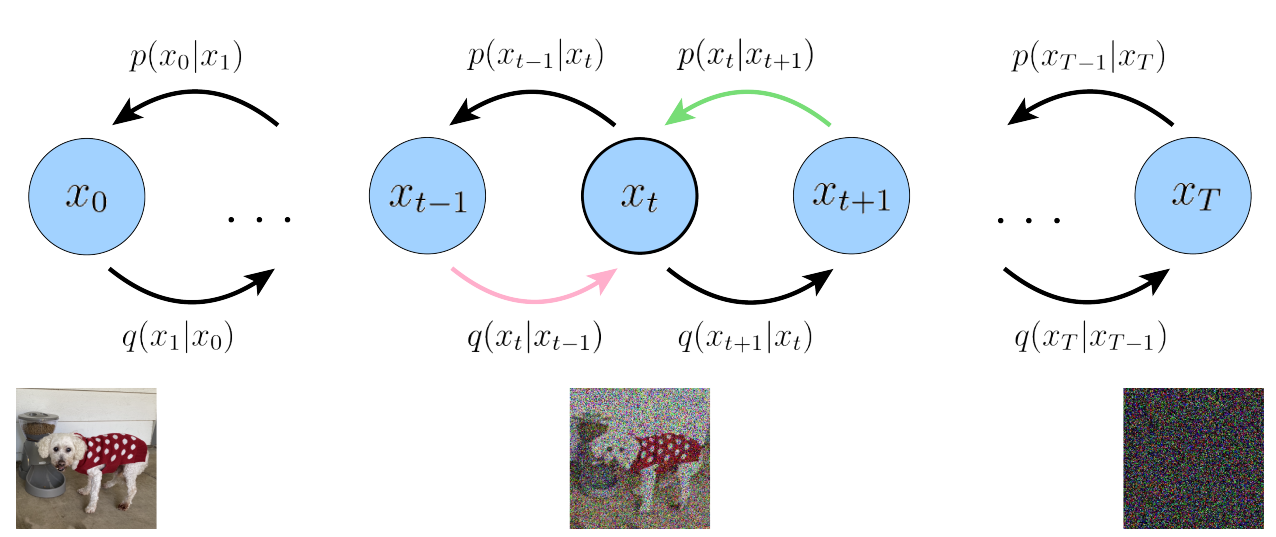
\includegraphics[width=\textwidth]{figures/diffusion_model_optimize_elbo}
    \caption{扩散模型证据下界一致检验项示意图}\label{fig:diffusion_model_optimize_elbo}
\end{figure}

图{\ref{fig:diffusion_model_optimize_elbo}}中,对于中间层隐变量{$\bm{x}_t$},
可以通过减小绿色箭头所代表的条件概率{$p(\bm{x}_{t}\mid \bm{x}_{t+1})$}与粉色箭头代表的高斯分布{$q(\bm{x}_{t}\mid \bm{x}_{t-1})$}的差异来优化,
由于需要对所有时间步骤{$t$}进行优化,扩散模型的优化时间取决于一致检验项。

式{\ref{eq:diffusion_elbo}}将证据下界分解为不同的期望项,
因此可以使用蒙特卡洛模拟来获得近似解,
但由于一致检验项在每个时间步计算关于两个随机变量{$\bm{x}_{t-1},\bm{x}_{t+1}$}的期望,
其蒙特卡洛估计的方差可能相比每个时间步只关于一个随机变量的项更高。
此外,由于需要对{$T-1$}步一致检验项进行求和,当{$T$}越大时,证据下界估计值的方差也越大。

由于马尔可夫性质,
{$\bm{x}_{t}$}不依赖于{$\bm{x}_{0}$},
可将编码过程改写为{$q(\bm{x}_{t}\mid \bm{x}_{t-1})=q(\bm{x}_{t}\mid \bm{x}_{t-1},\bm{x}_{0})$},
则根据贝叶斯定理可得:
\begin{equation}
    \label{eq:diffusion_rewrite_with_x_0}
    q(\bm{x}_{t}\mid \bm{x}_{t-1},\bm{x}_0)=\frac{q(\bm{x}_{t-1}\mid \bm{x}_{t},\bm{x}_0)q(\bm{x}_{t}\mid \bm{x}_0)}{q(\bm{x}_{t-1}\mid \bm{x}_0)}
\end{equation}
根据式{\ref{eq:diffusion_rewrite_with_x_0}},可由式{\ref{eq:diffusion_elbo_origin}}得:
\begin{align}
    &\log p(\bm{x})
    \\\geq &  \mathbb{E}_{q(\bm{x}_{1:T}\mid \bm{x}_0)} \left[ \log \frac{p(\bm{x}_{0:T})}{q(\bm{x}_{1:T}\mid \bm{x}_{0})}  \right]
    \\= &  \mathbb{E}_{q(\bm{x}_{1:T}\mid \bm{x}_0)} \left[ \log \frac{p(\bm{x}_{T})\prod_{t=1}^{T}{p_{\theta}(\bm{x}_{t-1}\mid \bm{x}_{t})}}{\prod_{t=1}^{T}q(\bm{x}_{t}\mid \bm{x}_{t-1})}  \right]
    \\= &  \mathbb{E}_{q(\bm{x}_{1:T}\mid \bm{x}_0)} \left[ \log \frac{p(\bm{x}_{T})p_{\theta}(\bm{x}_{0}\mid \bm{x}_{1})\prod_{t=2}^{T}{p_{\theta}(\bm{x}_{t-1}\mid \bm{x}_{t})}}{q(\bm{x}_{1}\mid \bm{x}_{0})\prod_{t=2}^{T}q(\bm{x}_{t}\mid \bm{x}_{t-1})}  \right]
    \\= &  \mathbb{E}_{q(\bm{x}_{1:T}\mid \bm{x}_0)} \left[ \log \frac{p(\bm{x}_{T})p_{\theta}(\bm{x}_{0}\mid \bm{x}_{1})\prod_{t=2}^{T}{p_{\theta}(\bm{x}_{t-1}\mid \bm{x}_{t})}}{q(\bm{x}_{1}\mid \bm{x}_{0})\prod_{t=2}^{T}q(\bm{x}_{t}\mid \bm{x}_{t-1},\bm{x}_{0})}  \right]
    \\= &  \mathbb{E}_{q(\bm{x}_{1:T}\mid \bm{x}_0)} \left[ \log \frac{p(\bm{x}_{T})p_{\theta}(\bm{x}_{0}\mid \bm{x}_{1})}{q(\bm{x}_{1}\mid \bm{x}_{0})} 
     + \log \prod_{t=2}^{T}\frac{p_{\theta}(\bm{x}_{t-1}\mid \bm{x}_{t})}{q(\bm{x}_{t}\mid \bm{x}_{t-1},\bm{x}_{0})} \right]
    \\= &  \mathbb{E}_{q(\bm{x}_{1:T}\mid \bm{x}_0)} \left[ \log \frac{p(\bm{x}_{T})p_{\theta}(\bm{x}_{0}\mid \bm{x}_{1})}{q(\bm{x}_{1}\mid \bm{x}_{0})} 
    + \log \prod_{t=2}^{T}\frac{p_{\theta}(\bm{x}_{t-1}\mid \bm{x}_{t})}{\frac{q(\bm{x}_{t-1}\mid \bm{x}_{t},\bm{x}_0)q(\bm{x}_{t}\mid \bm{x}_0)}{q(\bm{x}_{t-1}\mid \bm{x}_0)}} \right]
   \\= & \mathbb{E}_{q(\bm{x}_{1:T}\mid \bm{x}_0)} \left[ \log \frac{p(\bm{x}_{T})p_{\theta}(\bm{x}_{0}\mid \bm{x}_{1})}{q(\bm{x}_{1}\mid \bm{x}_{0})} 
   + \log \frac{q(\bm{x}_{1}\mid \bm{x}_{0})}{q(\bm{x}_{T}\mid \bm{x}_{0})}
   + \log \prod_{t=2}^{T}\frac{p_{\theta}(\bm{x}_{t-1}\mid \bm{x}_{t})}{q(\bm{x}_{t-1}\mid \bm{x}_{t},\bm{x}_0)} \right]
  \\= &  \mathbb{E}_{q(\bm{x}_{1:T}\mid \bm{x}_0)} \left[ \log \frac{p(\bm{x}_{T})p_{\theta}(\bm{x}_{0}\mid \bm{x}_{1})}{q(\bm{x}_{T}\mid \bm{x}_{0})} 
   + \sum_{t=2}^{T}\log \frac{p_{\theta}(\bm{x}_{t-1}\mid \bm{x}_{t})}{q(\bm{x}_{t-1}\mid \bm{x}_{t},\bm{x}_0)}\right]
   \\= & \mathbb{E}_{q(\bm{x}_{1:T}\mid \bm{x}_0)} \left[  \log p_{\theta}(\bm{x}_{0}\mid \bm{x}_{1}) \right]
   +  \mathbb{E}_{q(\bm{x}_{1:T}\mid \bm{x}_0)} \left[ \log \frac{p(\bm{x}_{T})}{q(\bm{x}_{T}\mid \bm{x}_{0})} \right]
   \nonumber \\ & \qquad+   \sum_{t=2}^{T} \mathbb{E}_{q(\bm{x}_{1:T}\mid \bm{x}_0)} \left[  \log \frac{p_{\theta}(\bm{x}_{t-1}\mid \bm{x}_{t})}{q(\bm{x}_{t-1}\mid \bm{x}_{t},\bm{x}_0)} \right]
   \\ &  = \mathbb{E}_{q(\bm{x}_{1}\mid \bm{x}_0)} \left[  \log p_{\theta}(\bm{x}_{0}\mid \bm{x}_{1}) \right]
   +  \mathbb{E}_{q(\bm{x}_{T}\mid \bm{x}_0)} \left[ \log \frac{p(\bm{x}_{T})}{q(\bm{x}_{T}\mid \bm{x}_{0})} \right]
   \nonumber \\ & \qquad+   \sum_{t=2}^{T} \mathbb{E}_{q(\bm{x}_{t},\bm{x}_{t-1}\mid \bm{x}_0)} \left[  \log \frac{p_{\theta}(\bm{x}_{t-1}\mid \bm{x}_{t})}{q(\bm{x}_{t-1}\mid \bm{x}_{t},\bm{x}_0)} \right]
   \\ &  = \underbrace{\mathbb{E}_{q(\bm{x}_{1}\mid \bm{x}_0)} \left[  \log p_{\theta}(\bm{x}_{0}\mid \bm{x}_{1}) \right]}_{\mbox{重构项}}
   - \underbrace{D_{KL}(q(\bm{x}_{T}\mid \bm{x}_{0}) \Vert p(\bm{x}_{T}))}_{\mbox{先验匹配项}}
   \nonumber \\ & \qquad - \sum_{t=2}^{T} \underbrace{\mathbb{E}_{q(\bm{x}_{t}\mid \bm{x}_0)} \left[ D_{KL}(q(\bm{x}_{t-1}\mid \bm{x}_{t},\bm{x}_0)\Vert p_{\theta}(\bm{x}_{t-1}\mid \bm{x}_{t}))  \right]}_{\mbox{降噪匹配项}} \label{eq:diffusion_elbo_expectation_single}
\end{align}

式{\ref{eq:diffusion_elbo_expectation_single}}相比式{\ref{eq:diffusion_elbo}},
每一项均为最多只关于一个随机变量的期望。
类比对式{\ref{eq:diffusion_elbo}}的解释,
式{\ref{eq:diffusion_elbo_expectation_single}}有如下解释:
\begin{itemize}
    \item {$\mathbb{E}_{q(\bm{x}_{1}\mid \bm{x}_0)} \left[  \log p_{\theta}(\bm{x}_{0}\mid \bm{x}_{1}) \right]$}
项为重构项,与变分自编码器证据下界中的重构项类似。可以蒙特卡洛模拟方法近似估计与优化。
\item {$D_{KL}(q(\bm{x}_{T}\mid \bm{x}_{0}) \Vert p(\bm{x}_{T}))$}项为先验匹配项,
表明不断添加噪声后的图像与高斯分布的匹配程度。
先验匹配项在扩散模型假设下为{$0$}。
\item {$ \mathbb{E}_{q(\bm{x}_{t}\mid \bm{x}_0)} \left[ D_{KL}(q(\bm{x}_{t-1}\mid \bm{x}_{t},\bm{x}_0)\Vert p_{\theta}(\bm{x}_{t-1}\mid \bm{x}_{t}))  \right] $ }
为降噪匹配项,
扩散模型用降噪变换{$p_{\theta}(\bm{x}_{t-1}\mid \bm{x}_{t})$}来近似真实降噪变换{$q(\bm{x}_{t-1}\mid \bm{x}_{t},\bm{x}_0)$}。
通过最小化降噪匹配项,
可以使两个降噪变换逐渐接近。
\end{itemize}
\begin{figure}[ht]
    \centering
    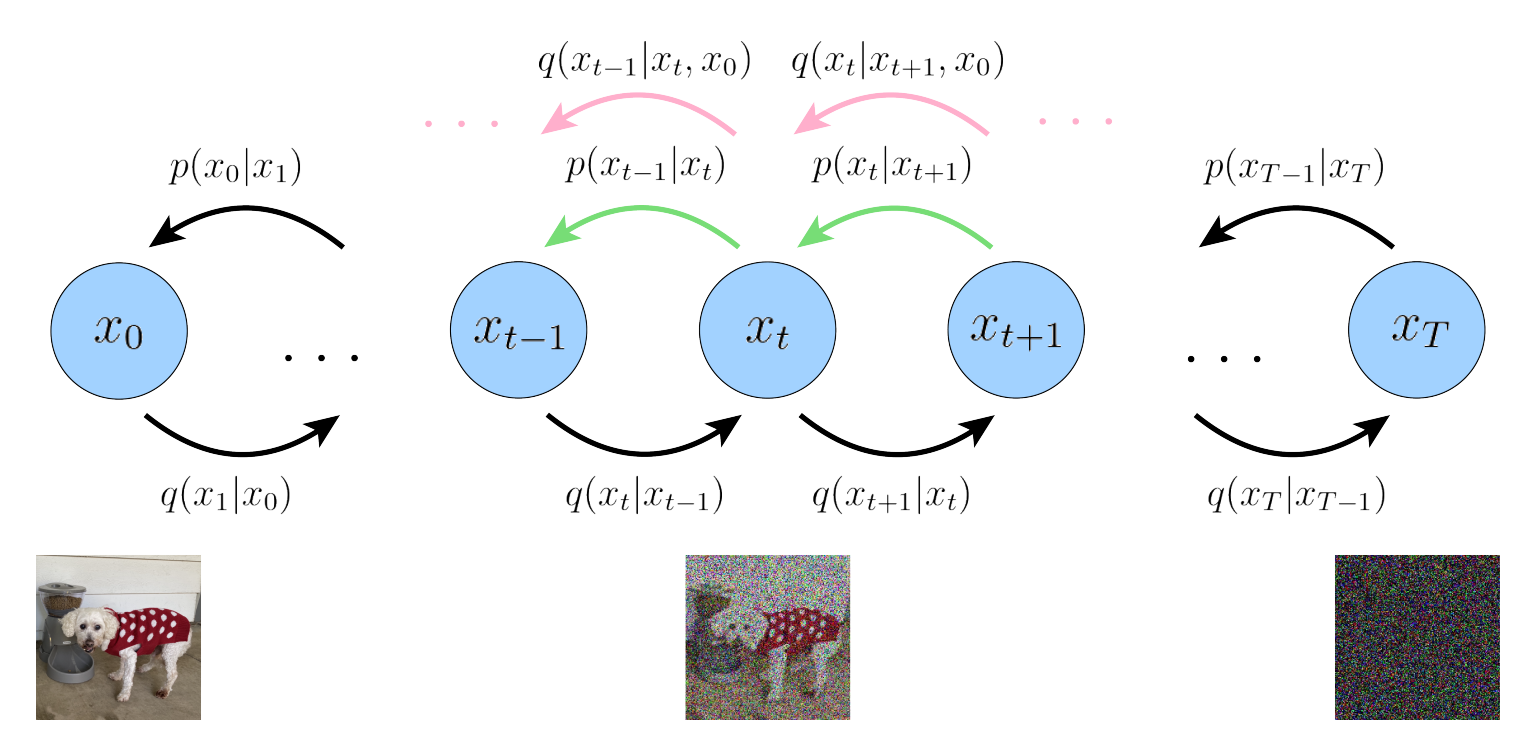
\includegraphics[width=\textwidth]{figures/diffusion_model_optimize_elbo_single_variable}
    \caption{扩散模型证据下界降噪匹配项单变量期望示意图}\label{fig:diffusion_model_optimize_elbo_single_variable}
\end{figure}

图{\ref{fig:diffusion_model_optimize_elbo_single_variable}}为使用式{\ref{eq:diffusion_elbo_expectation_single}}优化扩散模型示意图,
使用贝叶斯定理计算真实降噪过程{$q(\bm{x}_{t-1}\mid \bm{x}_{t},\bm{x}_0)$},
并计算其关于近似降噪过程{$p_{\theta}(\bm{x}_{t-1}\mid \bm{x}_{t})$}的KL散度,
即尽可能使绿色箭头所代表分布与粉色箭头所代表分布一致。

KL散度项{$D_{KL}(q(\bm{x}_{t-1}\mid \bm{x}_{t},\bm{x}_0)\Vert p_{\theta}(\bm{x}_{t-1}\mid \bm{x}_{t})) $}
由于需要同时对多个时间步的编码器进行学习,
难以进行最小化。
为使KL散度项更易优化,
根据贝叶斯定理有:
\begin{equation}
    \label{eq:diffusion_gaussion_transition_for_kl_divergence}
    q(\bm{x}_{t-1}\mid \bm{x}_{t},\bm{x}_0)=\frac{q(\bm{x}_{t}\mid \bm{x}_{t-1},\bm{x}_0) q(\bm{x}_{t-1}\mid \bm{x}_0)}{q(\bm{x}_{t}\mid \bm{x}_0) }
\end{equation}
根据式{\ref{eq:diffusion_encoder}},可得:
\begin{equation}
    \label{eq:diffusion_gaussion_transition_for_kl_divergence_likelihood}
    q(\bm{x}_{t}\mid \bm{x}_{t-1},\bm{x}_0)=q(\bm{x}_{t}\mid \bm{x}_{t-1})=\mathcal{N}(\bm{x}_{t}; \sqrt{\alpha}_{t}(\bm{x}_{t-1}), (1-\alpha_t)\bm{I})
\end{equation}
由于扩散模型编码器为线性高斯模型,
根据重参数方法,
对于{$\bm{x}_{t}\sim q(\bm{x}_{t},\bm{x}_{t-1})$}可得:
\begin{equation}
    \bm{x}_{t}=\sqrt{\alpha_{t}}\bm{x}_{t-1}+\sqrt{1-\alpha_{t}}\bm{\epsilon} \mbox{其中,} \epsilon \sim \mathcal{N}(\bm{\epsilon};\bm{0},\bm{I})
\end{equation}
对于{$\bm{x}_{t-1}\sim q(\bm{x}_{t-1},\bm{x}_{t-2})$}可得:
\begin{equation}
    \bm{x}_{t-1}=\sqrt{\alpha_{t-1}}\bm{x}_{t-2}+\sqrt{1-\alpha_{t-1}}\bm{\epsilon} \mbox{其中,} \epsilon \sim \mathcal{N}(\bm{\epsilon};\bm{0},\bm{I})
\end{equation}

可以使用重参数方法对{$q(\bm{x}_{t}\mid \bm{x}_{0})$}进行递归推导,
假设有{$2T$}个随机噪声变量{$\{\bm{\epsilon}_{t}^{*},\bm{\epsilon}_{t}\}_{t=0}^{T} \stackrel {iid} \sim \mathcal{N}(\bm{\epsilon;\bm{0},\bm{I}})$},
则对于任意采样{$\bm{x}_{t}\sim q(\bm{x}_{t}\mid \bm{x}_{0})$},有:
\begin{align}
    \bm{x}_{t}
    &=\sqrt{\alpha_{t}}\bm{x}_{t-1} +\sqrt{1-\alpha_{t}}\bm{\epsilon}_{t-1}^{*}
    \\ & = \sqrt{\alpha}_{t}(  \sqrt{\alpha}_{t-1} \bm{x}_{t-2} +\sqrt{1-\alpha_{t-1}}\bm{\epsilon}_{t-2}^{*}  ) +\sqrt{1-\alpha_{t}}\bm{\epsilon}_{t-1}^{*}
    \\ & = \sqrt{\alpha_{t}\alpha_{t-1}}\bm{x}_{t-2}  + \sqrt{\alpha_{t}-\alpha_{t}\alpha_{t-1}}\bm{\epsilon}_{t-2}^{*} +\sqrt{1-\alpha_{t}}\bm{\epsilon}_{t-1}^{*}
    \\ & = \sqrt{\alpha_{t}\alpha_{t-1}}\bm{x}_{t-2}  + \sqrt{\sqrt{{\alpha_{t}-\alpha_{t}\alpha_{t-1}}}^{2}+{\sqrt{1-\alpha_{t}}}^{2}}\bm{\epsilon}_{t-2} \mbox{\qquad 根据式{\ref{eq:sum_of_two_gaussian_distributions}}}
    \\ & = \sqrt{\alpha_{t}\alpha_{t-1}}\bm{x}_{t-2}  +\sqrt{\alpha_{t}-\alpha_{t}\alpha_{t-1} + 1-\alpha_{t}} \bm{\epsilon}_{t-2}
    \\ & =\sqrt{\alpha_{t}\alpha_{t-1}}\bm{x}_{t-2}  +\sqrt{1-\alpha_{t}\alpha_{t-1} } \bm{\epsilon}_{t-2}
    \\ & = \ldots
    \\ & = \sqrt{\prod_{i=1}^{t}\alpha_{i}}\bm{x}_{0}+ \sqrt{1- \prod_{i=1}^{t}\alpha_{i}}\bm{\epsilon}_{0}
    \\ & = \sqrt{\bar{\alpha}_{t}}\bm{x}_{0} +\sqrt{1- \bar{\alpha}_{t}}\bm{\epsilon}_{0}
    \\ & \sim \mathcal{N}(\bm{x}_{t}; \sqrt{\bar{\alpha}_{t}}\bm{x}_{0},(1- \bar{\alpha}_{t})\bm{I}) \label{eq:diffusion_x_t_gaussian_distribution}
\end{align}
与式{\ref{eq:diffusion_x_t_gaussian_distribution}}类似,有:
\begin{equation}
    \label{eq:diffusion_x_t_minux_1_gaussian_distribution}
    \bm{x}_{t-1} \sim \mathcal{N}(\bm{x}_{t-1}; \sqrt{\bar{\alpha}_{t-1}}\bm{x}_{0},(1- \bar{\alpha}_{t-1})\bm{I})
\end{equation}

由式{\ref{eq:diffusion_gaussion_transition_for_kl_divergence}}、
式{\ref{eq:diffusion_gaussion_transition_for_kl_divergence_likelihood}}、
式{\ref{eq:diffusion_x_t_gaussian_distribution}}和式{\ref{eq:diffusion_x_t_minux_1_gaussian_distribution}},
可得:
\begin{align}
    &q(\bm{x}_{t-1}\mid \bm{x}_{t},\bm{x}_0)
    \\ = &\frac{q(\bm{x}_{t}\mid \bm{x}_{t-1},\bm{x}_0) q(\bm{x}_{t-1}\mid \bm{x}_0)}{q(\bm{x}_{t}\mid \bm{x}_0) }
    \\  \propto & \exp \{ -\frac{1}{2}  \left[   \frac{{(\bm{x}_{t}-\sqrt{\alpha_{t}}\bm{x}_{t-1})}^{2}}{1-\alpha_{t}}
    +  \frac{{(\bm{x}_{t-1}-\sqrt{\bar{\alpha}_{t-1}}\bm{x}_{0})}^{2}}{1-\bar{\alpha}_{t-1}}
    - \frac{{(\bm{x}_{t}-\sqrt{\bar{\alpha}_{t}}\bm{x}_{0})}^{2}}{1-\bar{\alpha}_{t}}
     \right]  \}
    \\ = & \exp \{ -\frac{1}{2}  \left[ 
    \frac{-2 \sqrt{\alpha_{t}}\bm{x}_{t}\bm{x}_{t-1}+\alpha_{t}\bm{x}_{t-1}^{2}}{1-\alpha_{t}}
     +  \frac{{(\bm{x}_{t-1}^{2} -2\sqrt{\bar{\alpha}_{t-1}}\bm{x}_{t-1}\bm{x}_{0})}^{2}}{1-\bar{\alpha}_{t-1}}
     + C(\bm{x}_{t},\bm{x}_{0})
        \right]  \} \label{eq:diffusion_kl_divergence_q_with_c}
    \\  \propto & \exp \{ -\frac{1}{2}  \left[ 
        -\frac{2 \sqrt{\alpha_{t}}\bm{x}_{t}\bm{x}_{t-1}}{1-\alpha_{t}}
        +\frac{\alpha_{t}\bm{x}_{t-1}^{2}}{1-\alpha_{t}}
        + \frac{\bm{x}_{t-1}^{2} }{1-\bar{\alpha}_{t-1}}
        - \frac{2\sqrt{\bar{\alpha}_{t-1}}\bm{x}_{t-1}\bm{x}_{0}}{1-\bar{\alpha}_{t-1}}
         \right]  \}
    \\ = & \exp \{ -\frac{1}{2}  \left[ 
    \left(\frac{\alpha_{t}}{1-\alpha_{t}}+ \frac{1}{1-\bar{\alpha}_{t-1}}\right) \bm{x}_{t-1}^{2}
    -2\left(\frac{\sqrt{\alpha_{t}}\bm{x}_{t}}{1-\alpha_{t}}  + \frac{\sqrt{\bar{\alpha}_{t-1}}\bm{x}_{0}}{1-\bar{\alpha}_{t-1}}  \right)\bm{x}_{t-1}
        \right]  \}
    \\ = & \exp \{ -\frac{1}{2}  \left[ 
    \frac{\alpha_{t}(1-\bar{\alpha}_{t-1})+1-\alpha_{t}}{(1-\alpha_{t})(1-\bar{\alpha}_{t-1})} \bm{x}_{t-1}^{2}
    -2\left(\frac{\sqrt{\alpha_{t}}\bm{x}_{t}}{1-\alpha_{t}}  + \frac{\sqrt{\bar{\alpha}_{t-1}}\bm{x}_{0}}{1-\bar{\alpha}_{t-1}}  \right)\bm{x}_{t-1}
        \right]  \}
    \\ = & \exp \{ -\frac{1}{2}  \left[ 
    \frac{\alpha_{t}-\bar{\alpha}_{t}+1-\alpha_{t}}{(1-\alpha_{t})(1-\bar{\alpha}_{t-1})} \bm{x}_{t-1}^{2}
    -2\left(\frac{\sqrt{\alpha_{t}}\bm{x}_{t}}{1-\alpha_{t}}  + \frac{\sqrt{\bar{\alpha}_{t-1}}\bm{x}_{0}}{1-\bar{\alpha}_{t-1}}  \right)\bm{x}_{t-1}
        \right]  \}
    \\ = & \exp \{ -\frac{1}{2}  \left[ 
    \frac{1-\bar{\alpha}_{t}}{(1-\alpha_{t})(1-\bar{\alpha}_{t-1})} \bm{x}_{t-1}^{2}
    -2\left(\frac{\sqrt{\alpha_{t}}\bm{x}_{t}}{1-\alpha_{t}}  + \frac{\sqrt{\bar{\alpha}_{t-1}}\bm{x}_{0}}{1-\bar{\alpha}_{t-1}}  \right)\bm{x}_{t-1}
        \right]  \}
    \\ = & \exp \{ -\frac{1}{2} \left(    \frac{1-\bar{\alpha}_{t}}{(1-\alpha_{t})(1-\bar{\alpha}_{t-1})} \right) \left[ 
   \bm{x}_{t-1}^{2}
   -2\frac{\left(\frac{\sqrt{\alpha_{t}}\bm{x}_{t}}{1-\alpha_{t}}  + \frac{\sqrt{\bar{\alpha}_{t-1}}\bm{x}_{0}}{1-\bar{\alpha}_{t-1}}  \right)}{  \frac{1-\bar{\alpha}_{t}}{(1-\alpha_{t})(1-\bar{\alpha}_{t-1})}}\bm{x}_{t-1}
        \right]  \}
    \\ = & \exp \{ -\frac{1}{2} \left(    \frac{1-\bar{\alpha}_{t}}{(1-\alpha_{t})(1-\bar{\alpha}_{t-1})} \right)
    \nonumber \\ & \qquad \qquad \left[ 
   \bm{x}_{t-1}^{2}
   -2\frac{\left(\frac{\sqrt{\alpha_{t}}\bm{x}_{t}}{1-\alpha_{t}}  + \frac{\sqrt{\bar{\alpha}_{t-1}}\bm{x}_{0}}{1-\bar{\alpha}_{t-1}}  \right)(1-\alpha_{t})(1-\bar{\alpha}_{t-1})}{  1-\bar{\alpha}_{t}}\bm{x}_{t-1}
        \right]  \}
    \\ = & \exp \{ -\frac{1}{2} \left(    \frac{1}{\frac{(1-\alpha_{t})(1-\bar{\alpha}_{t-1})}{1-\bar{\alpha}_{t}}} \right) \left[ 
   \bm{x}_{t-1}^{2}
   -2\frac{\sqrt{\alpha_{t}}(1-\bar{\alpha}_{t-1})\bm{x}_{t} + \sqrt{\bar{\alpha}_{t-1}}(1-\alpha_{t})\bm{x}_{0}}{  1-\bar{\alpha}_{t}}\bm{x}_{t-1}
        \right]  \} \label{eq:diffusion_kl_divergence_q_distribution_no_complete_square}
    \\ \propto  & \mathcal{N}(\bm{x}_{t-1};
    \underbrace{\frac{\sqrt{\alpha_{t}}(1-\bar{\alpha}_{t-1})\bm{x}_{t} + \sqrt{\bar{\alpha}_{t-1}}(1-\alpha_{t})\bm{x}_{0}}{  1-\bar{\alpha}_{t}}}_{\mu_{q}(\bm{x}_{t},\bm{x}_{0})},
    \underbrace{\frac{(1-\alpha_{t})(1-\bar{\alpha}_{t-1})}{1-\bar{\alpha}_{t}}\bm{I}}_{\bm{\Sigma}_{q}(t)}) \label{eq:diffusion_kl_divergence_q_distribution}
\end{align}

式{\ref{eq:diffusion_kl_divergence_q_with_c}}中,{$C(\bm{x}_{t},\bm{x}_{0})$}为由{$\bm{x}_{t},\bm{x}_{0},\alpha$}组成的相对于{$\bm{x}_{t-1}$}的常数项,
可与式{\ref{eq:diffusion_kl_divergence_q_distribution_no_complete_square}}经过配方法式{\ref{eq:completing_the_square_method}},
获得式{\ref{eq:diffusion_kl_divergence_q_distribution}}。
即{$\bm{x}_{t-1} \sim q(\bm{x}_{t-1}\mid \bm{x}_{t},\bm{x}_{0})$}为正态分布,
均值{$\mu_{q}(\bm{x}_{t},\bm{x}_{0})$}为{$\bm{x}_{t},\bm{x}_{0}$}的函数,
方差{$\bm{\Sigma}_{q}(t)$}为{$\alpha$}的函数,
{$\alpha$}为已知的关于时间步的确定量,
可以为超参数或由神经网络学习获得。
根据式{\ref{eq:diffusion_kl_divergence_q_distribution}},
可得:
\begin{equation}
    \label{eq:diffusion_q_sigma}
    \Sigma_{q}(t)= \sigma_{q}^{2}(t)\bm{I}= \frac{(1-\alpha_{t})(1-\bar{\alpha}_{t-1})}{1-\bar{\alpha}_{t}}\bm{I}
\end{equation}

为使近似降噪转换{$p_{\theta}(\bm{x}_{t-1}\mid \bm{x}_{t})$}与真实降噪转换{$q(\bm{x}_{t-1}\mid \bm{x}_{t},\bm{x}_{0})$}更加接近,
可以使{$p_{\theta}(\bm{x}_{t-1}\mid \bm{x}_{t})$}服从高斯分布。
此外,由于{$\alpha$}在转换过程中为固定值,
可以令近似降噪转换的方差与真实降噪转换的方差相同,即{$\bm{\Sigma}_{q}(t)= \sigma_{q}^{2}(t)\bm{I}$}。
而对于高斯分布的均值,由于真实降噪转换的高斯分布均值{$\mu_{q}(\bm{x}_{t},\bm{x}_{0})$}为{$\bm{x}_{t},\bm{x}_{0}$}的函数,
近似降噪转换{$p_{\theta}(\bm{x}_{t-1}\mid \bm{x}_{t})$}却不含有{$\bm{x}_{0}$},
可将近似降噪转换高斯分布的均值设为{$\bm{\mu}_{\theta}(\bm{x}_{t},t)$}。

根据两高斯分布KL散度计算式{\ref{eq:kl_divergence_of_two_gaussian}},
由于近似降噪转换的方差与真实降噪转换的方差相同,
最小化KL散度即转换为最小化两分布的均值,即:
\begin{align}
    &\argmin_{\theta} D_{KL}(q(\bm{x}_{t-1}\mid \bm{x}_{t},\bm{x}_{0}) \Vert p_{\theta}(\bm{x}_{t-1}\mid \bm{x}_{t})  )
    \\=& \argmin_{\theta}  D_{KL}(\mathcal{N}(\bm{x}_{t-1};\bm{\mu}_{q},\bm{\Sigma}_{q}(t))\Vert \mathcal{N}(\bm{x}_{t-1};\bm{\mu}_{\theta},\bm{\Sigma}_{q}(t)))
    \\=& \argmin_{\theta}  \frac{1}{2}\left[
        \log \frac{\left|  \bm{\Sigma}_{q}(t) \right|}{\left|  \bm{\Sigma}_{q}(t) \right|}
        - d
        +tr({\bm{\Sigma}_{q}(t)}^{-1}\bm{\Sigma}_{q}(t))
        +{(\bm{\mu}_{\theta}-\bm{\mu}_{q})}^{\intercal}{\bm{\Sigma}_{q}(t)}^{-1}(\bm{\mu}_{\theta}-\bm{\mu}_{q})
    \right]
    \\=& \argmin_{\theta}  \frac{1}{2}\left[\log 1 -d +d + {(\bm{\mu}_{\theta}-\bm{\mu}_{q})}^{\intercal}{\bm{\Sigma}_{q}(t)}^{-1}(\bm{\mu}_{\theta}-\bm{\mu}_{q})\right]
    \\=& \argmin_{\theta}  \frac{1}{2}\left[{(\bm{\mu}_{\theta}-\bm{\mu}_{q})}^{\intercal}{\bm{\Sigma}_{q}(t)}^{-1}(\bm{\mu}_{\theta}-\bm{\mu}_{q})\right]
    \\=& \argmin_{\theta}  \frac{1}{2}\left[{(\bm{\mu}_{\theta}-\bm{\mu}_{q})}^{\intercal}{\sigma_{q}^{2}(t)\bm{I}}^{-1}(\bm{\mu}_{\theta}-\bm{\mu}_{q})\right]
    \\=& \argmin_{\theta}  \frac{1}{2(\sigma_{q}^{2}(t))}\left[ {\Vert \bm{\mu}_{\theta}-\bm{\mu}_{q} \Vert}_{2}^{2}  \right] \label{eq:diffusion_kl_divergence_two_gaussian_mu}
\end{align}

式{\ref{eq:diffusion_kl_divergence_two_gaussian_mu}}中,
{$\bm{\mu}_{q}$}为{$\bm{\mu}_{q}(\bm{x}_{t},\bm{x}_{0})$}的缩写,
{$\bm{\mu}_{\theta}$}为{$\bm{\mu}_{\theta}(\bm{x}_{t},t)$}的缩写。
由式{\ref{eq:diffusion_kl_divergence_q_distribution}},真实降噪转换分布的均值为:
\begin{equation}
    \label{diffusion_mu_}
    \bm{\mu}_{q}(\bm{x}_{t},\bm{x}_{0})=\frac{\alpha_{t}(1-\bar{\alpha}_{t-1})\bm{x}_{t} + \sqrt{\bar{\alpha}_{t-1}}1-\alpha_{t}\bm{x}_{0}}{  1-\bar{\alpha}_{t}}
\end{equation}

为使近似降噪转换的均值{$\bm{\mu}_{\theta}(\bm{x}_{t},t)$}与真实降噪转换的均值{$\bm{\mu}_{q}(\bm{x}_{t},\bm{x}_{0})$}的均值尽可能一致,
由于近似降噪转换的均值{$\bm{\mu}_{\theta}(\bm{x}_{t},t)$}也包含{$\bm{x}_{t}$},可令两均值具有相似形式,即:
\begin{equation}
    \label{eq:diffusion_mu_theta}
    \bm{\mu}_{\theta}(\bm{x}_{t},t)=\frac{\alpha_{t}(1-\bar{\alpha}_{t-1})\bm{x}_{t} + \sqrt{\bar{\alpha}_{t-1}}1-\alpha_{t}\hat{\bm{x}}_{\theta}(\bm{x}_{t},t)}{  1-\bar{\alpha}_{t}}
\end{equation}

式{\ref{eq:diffusion_mu_theta}}中,
{$\hat{\bm{x}}_{\theta}(\bm{x}_{t},t)$}为由噪声图像{$\bm{x}_{t}$}和时间索引{$t$}预测原始样本{$\bm{x}_{0}$}的神经网络。
则优化问题可转化为:
\begin{align}
    &\argmin_{\theta} D_{KL}(q(\bm{x}_{t-1}\mid \bm{x}_{t},\bm{x}_{0}) \Vert p_{\theta}(\bm{x}_{t-1}\mid \bm{x}_{t})  )
    \\=& \argmin_{\theta}  D_{KL}(\mathcal{N}(\bm{x}_{t-1};\bm{\mu}_{q},\bm{\Sigma}_{q}(t))\Vert \mathcal{N}(\bm{x}_{t-1};\bm{\mu}_{\theta},\bm{\Sigma}_{q}(t)))
    \\=& \argmin_{\theta}  \frac{1}{2(\sigma_{q}^{2}(t))}\left[ {\Vert \bm{\mu}_{\theta}-\bm{\mu}_{q} \Vert}_{2}^{2}  \right] 
    \\=& \argmin_{\theta}  \frac{1}{2(\sigma_{q}^{2}(t))}\left[ \left\Vert 
    \frac{\alpha_{t}(1-\bar{\alpha}_{t-1})\bm{x}_{t} + \sqrt{\bar{\alpha}_{t-1}}1-\alpha_{t}\bm{x}_{0}}{  1-\bar{\alpha}_{t}}
    \right. \right. \\ & \qquad \qquad \left. \left. -\frac{\alpha_{t}(1-\bar{\alpha}_{t-1})\bm{x}_{t} + \sqrt{\bar{\alpha}_{t-1}}1-\alpha_{t}\hat{\bm{x}}_{\theta}(\bm{x}_{t},t)}{  1-\bar{\alpha}_{t}}
    \right\Vert_{2}^{2} \right]
    \\=& \argmin_{\theta}  \frac{1}{2(\sigma_{q}^{2}(t))}\left[ {\left\Vert 
    \frac{ \sqrt{\bar{\alpha}_{t-1}}(1-\alpha_{t})\hat{\bm{x}}_{\theta}(\bm{x}_{t}, t)}{  1-\bar{\alpha}_{t}}
    -\frac{\sqrt{\bar{\alpha}_{t-1}}1-\alpha_{t}\bm{x}_{0}}{  1-\bar{\alpha}_{t}}
    \right\Vert}_{2}^{2} \right]
    \\=& \argmin_{\theta}  \frac{1}{2(\sigma_{q}^{2}(t))}\left[ {\left\Vert 
    \frac{ \sqrt{\bar{\alpha}_{t-1}}(1-\alpha_{t})}{  1-\bar{\alpha}_{t}}
    (\hat{\bm{x}}_{\theta}(\bm{x}_{t}, t)-\bm{x}_{0})
    \right\Vert}_{2}^{2} \right]
    \\=& \argmin_{\theta}  \frac{1}{2(\sigma_{q}^{2}(t))}
    \frac{\bar{\alpha}_{t-1}{(1-\alpha_{t})}^{2}}{{ 1-\bar{\alpha}_{t}}^{2}}\left[ {\left\Vert
    \hat{\bm{x}}_{\theta}(\bm{x}_{t}, t)-\bm{x}_{0}
    \right\Vert}_{2}^{2}\right] \label{eq:diffusion_optimize}
\end{align}

由式{\ref{eq:diffusion_optimize}},对扩散模型的优化可以转化为对神经网络的训练,
该神经网络可以从任意时刻噪声图像来预测真实样本。
此外,对式{\ref{eq:diffusion_elbo_expectation_single}}中的降噪匹配求和项,
可以通过最小化所有时刻的期望{$\eta$} 来近似,即:
\begin{equation}
    \label{eq:diffusion_minimize_expectation_over_all_timesteps_for_sum_of_denoising_Matching}
    \argmin_{\theta}\mathbb{E}_{t\sim U\{2,T\}}\left[
         \mathbb{E}_{q(\bm{x}_{t}\mid \bm{x}_0)} \left[ D_{KL}(q(\bm{x}_{t-1}\mid \bm{x}_{t},\bm{x}_0)\Vert p_{\theta}(\bm{x}_{t-1}\mid \bm{x}_{t}))  \right]
    \right]
\end{equation}

噪声参数{$\alpha_{t}$}可设置为超参数,也可参与训练学习获得。
可以使用以{$\eta$}为参数的神经网络{$\hat{\alpha}_{\bm{\eta}}(t)$}来获得{$\alpha_{t}$},
但由于每个时间步{$t$}都需计算{$\alpha_{t}$},效率较低,
可将式{\ref{eq:diffusion_q_sigma}}代入式{\ref{eq:diffusion_optimize}},
可得:
\begin{align}
    &\frac{1}{2(\sigma_{q}^{2}(t))}
    \frac{\bar{\alpha}_{t-1}{(1-\alpha_{t})}^{2}}{{ 1-\bar{\alpha}_{t}}^{2}}\left[ {\left\Vert
    \hat{\bm{x}}_{\theta}(\bm{x}_{t}, t)-\bm{x}_{0}
    \right\Vert}_{2}^{2}\right]
    \\ = & \frac{1}{2\frac{(1-\alpha_{t})(1-\bar{\alpha}_{t-1})}{1-\bar{\alpha}_{t}}}
    \frac{\bar{\alpha}_{t-1}{(1-\alpha_{t})}^{2}}{{ 1-\bar{\alpha}_{t}}^{2}}\left[ {\left\Vert
    \hat{\bm{x}}_{\theta}(\bm{x}_{t}, t)-\bm{x}_{0}
    \right\Vert}_{2}^{2}\right]
    \\ = & \frac{1}{2}\frac{1-\bar{\alpha}_{t}}{(1-\alpha_{t})(1-\bar{\alpha}_{t-1})}
    \frac{\bar{\alpha}_{t-1}{(1-\alpha_{t})}^{2}}{{ 1-\bar{\alpha}_{t}}^{2}}\left[ {\left\Vert
    \hat{\bm{x}}_{\theta}(\bm{x}_{t}, t)-\bm{x}_{0}
    \right\Vert}_{2}^{2}\right]
    \\ = & \frac{1}{2}
    \frac{\bar{\alpha}_{t-1}(1-\alpha_{t})}{(1-\bar{\alpha}_{t-1})(1-\bar{\alpha}_{t})}
    \left[ {\left\Vert
    \hat{\bm{x}}_{\theta}(\bm{x}_{t}, t)-\bm{x}_{0}
    \right\Vert}_{2}^{2}\right]
    \\ = & \frac{1}{2}
    \frac{\bar{\alpha}_{t-1}-\bar{\alpha}_{t}}{(1-\bar{\alpha}_{t-1})(1-\bar{\alpha}_{t})}
    \left[ {\left\Vert
    \hat{\bm{x}}_{\theta}(\bm{x}_{t}, t)-\bm{x}_{0}
    \right\Vert}_{2}^{2}\right]
    \\ = & \frac{1}{2}
    \frac{\bar{\alpha}_{t-1}
    -\bar{\alpha}_{t}\bar{\alpha}_{t-1}+\bar{\alpha}_{t}\bar{\alpha}_{t-1}
    -\bar{\alpha}_{t}}
    {(1-\bar{\alpha}_{t-1})(1-\bar{\alpha}_{t})}
    \left[ {\left\Vert
    \hat{\bm{x}}_{\theta}(\bm{x}_{t}, t)-\bm{x}_{0}
    \right\Vert}_{2}^{2}\right]
    \\ = & \frac{1}{2}
    \frac{\bar{\alpha}_{t-1}(1-\bar{\alpha}_{t})-\bar{\alpha}_{t}(1-\bar{\alpha}_{t-1})}
    {(1-\bar{\alpha}_{t-1})(1-\bar{\alpha}_{t})}
    \left[ {\left\Vert
    \hat{\bm{x}}_{\theta}(\bm{x}_{t}, t)-\bm{x}_{0}
    \right\Vert}_{2}^{2}\right]
    \\ = & \frac{1}{2}\left(
        \frac{\bar{\alpha}_{t-1}(1-\bar{\alpha}_{t})}{(1-\bar{\alpha}_{t-1})(1-\bar{\alpha}_{t})}
        -\frac{\bar{\alpha}_{t}(1-\bar{\alpha}_{t-1})}{(1-\bar{\alpha}_{t-1})(1-\bar{\alpha}_{t})}
    \right)
    \left[ {\left\Vert
    \hat{\bm{x}}_{\theta}(\bm{x}_{t}, t)-\bm{x}_{0}
    \right\Vert}_{2}^{2}\right]
    \\ = & \frac{1}{2}\left(
        \frac{\bar{\alpha}_{t-1}}{1-\bar{\alpha}_{t-1}}
        -\frac{\bar{\alpha}_{t}}{1-\bar{\alpha}_{t}}
    \right)
    \left[ {\left\Vert
    \hat{\bm{x}}_{\theta}(\bm{x}_{t}, t)-\bm{x}_{0}
    \right\Vert}_{2}^{2}\right] \label{eq:diffusion_learning_diffusion_noise_parameters}
\end{align}

根据式{\ref{eq:diffusion_x_t_gaussian_distribution}},
{$q(\bm{x}_{t}\mid \bm{x}_{0})$}为服从高斯分布{$\mathcal{N}(\bm{x}_{t}; \sqrt{\bar{\alpha}_{t}}\bm{x}_{0},(1- \bar{\alpha}_{t})\bm{I})$},
则根据信噪比定义式{\ref{eq:signal_to_noise_ratio}}可得:
\begin{equation}
    \label{eq:diffusion_snr}
    SNR(t)=\frac{\bar{\alpha}_{t}}{1-\bar{\alpha}_{t}}
\end{equation}

根据式{\ref{eq:diffusion_snr}}可将式{\ref{eq:diffusion_learning_diffusion_noise_parameters}}改写为:
\begin{align}
    &\frac{1}{2(\sigma_{q}^{2}(t))}
    \frac{\bar{\alpha}_{t-1}{(1-\alpha_{t})}^{2}}{{ 1-\bar{\alpha}_{t}}^{2}}\left[ {\left\Vert
    \hat{\bm{x}}_{\theta}(\bm{x}_{t}, t)-\bm{x}_{0}
    \right\Vert}_{2}^{2}\right]
    \\ = &  \frac{1}{2}\left(
        \frac{\bar{\alpha}_{t-1}}{1-\bar{\alpha}_{t-1}}
        -\frac{\bar{\alpha}_{t}}{1-\bar{\alpha}_{t}}
    \right)
    \left[ {\left\Vert
    \hat{\bm{x}}_{\theta}(\bm{x}_{t}, t)-\bm{x}_{0}
    \right\Vert}_{2}^{2}\right] 
    \\ = &  \frac{1}{2}\left(
        SNR(t-1)-SNR(t)
    \right)
    \left[ {\left\Vert
    \hat{\bm{x}}_{\theta}(\bm{x}_{t}, t)-\bm{x}_{0}
    \right\Vert}_{2}^{2}\right] \label{eq:diffusion_learning_difufsion_noise_parameters_snr}
\end{align}

根据信噪比定义,信噪比越高,则包含更多的信息,信噪比越低,则噪声越多。
扩散模型的信噪比随着时间步{$t$}的增加而单调减小,
即{$\bm{x}_{t}$}随着时间推移而逐渐包含更多的噪声,
直至在{$t=T$}时变为标准高斯分布。

为简化式{\ref{eq:diffusion_learning_difufsion_noise_parameters_snr}},
可使用神经网络来模拟任意时间的信噪比,并与扩散模型同时训练。即:
\begin{equation}
    \label{eq:diffusion_snr_nn}
    SNR(t)=\exp(-\omega_{\bm{\eta}}(t))
\end{equation}

式{\ref{eq:diffusion_snr_nn}}中,
{$\omega_{\bm{\eta}}(t)$}为单调递增函数,
{$-\omega_{\bm{\eta}}(t)$}为单调递减函数,
进行指数化以使信噪比为正数。
此时,使用神经网络模拟任意时间信噪比,式{\ref{eq:diffusion_minimize_expectation_over_all_timesteps_for_sum_of_denoising_Matching}}需要同时对{$\bm{\eta}$}进行优化。

此外,由式{\ref{eq:diffusion_snr}}、式{\ref{eq:diffusion_snr_nn}}和式{\ref{eq:sigmoid_function}},
可得:
\begin{align}
    \frac{\bar{\alpha}_{t}}{1-\bar{\alpha}_{t}} & =\exp(-\omega_{\bm{\eta}}(t)) \\
    \bar{\alpha}_{t} & = sigmoid(-\omega_{\bm{\eta}}(t)) \label{eq:diffusion_bar_alpha_t}\\
    1-\bar{\alpha}_{t} & = sigmoid(\omega_{\bm{\eta}}(t)) \label{eq:diffusion_bar_1_minux_bar_alpha_t}
\end{align}

式{\ref{eq:diffusion_bar_alpha_t}}和式{\ref{eq:diffusion_bar_1_minux_bar_alpha_t}}可用于
式{\ref{eq:diffusion_kl_divergence_q_distribution_no_complete_square}}中使用重参数方法从原始样本{$\bm{x}_{0}$}生成任意时刻添加噪声后的图像{$\bm{x}_{t}$}。



%%%%%%%%%%%%%%%%%%%%%%%%%%%%%%%%%%%%%%%%%%%%%%%%%%%%%%%%%%%%%%%%%%%%%%%DIFFUSIONDIFFUSION





\section{隐式密度模型}\label{section:implicit_density_model}
隐式密度模型不定义概率密度函数{$p_{model}(\bm{x};\bm{\theta})$},
不通过最大化似然函数来训练,
而通过其他方式与实际概率密度函数{$p_{data}$}进行交互。
\subsection{生成对抗网络}
生成对抗网络可以视为根据博弈论设计的一场游戏,
包含两个机器学习模型,
机器学习模型通常采用神经网络。

其中一个神经网络为生成器,
其隐式地确定了概率分布{$p_{model}$},
生成器不需要对概率分布{$p_{model}$}进行评估。
根据一个先验分布{$p(\bm{z})$}以及生成函数方程{$G(\bm{z};\theta^{(G)})$},
生成器可以从概率分布{$p_{model}$}中采样,
其中可学习参数{$\theta^{(G)}$}确定了生成器在博弈中采取的策略,
先验分布{$p(\bm{z})$}经常为相对而言无特殊结构的分布,
比如高维高斯分布或超立方体均匀分布,
从这类分布中采样的{$\bm{z}$}为随机噪声。
生成器的主要任务是通过学习将随机噪声{$\bm{z}$}转化为能够以假乱真的样本。

另一个神经网络为辨别器,
辨别器可以通过辨别函数{$D(\bm{x};\bm{\theta}^{(D)})$},
判断一个样本{$x$}是从训练集中采样的真实样本或是由生成器生成的伪造样本。





\begin{figure}[ht]
    \centering
    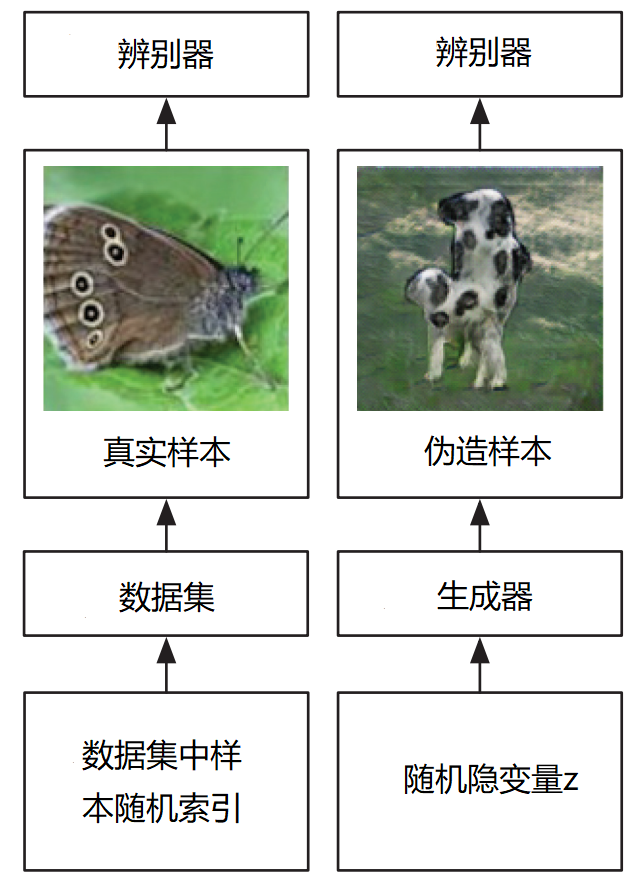
\includegraphics[height=0.5\textheight]{figures/gan_training}
    \caption{生成对抗网络训练过程}\label{fig:gan_training}
\end{figure}

图{\ref{fig:gan_training}}为生成对抗网络训练过程,
生成对抗网络的训练包括两部分:
对生成网络的训练和对辨别网络的训练。
训练的过程包括不断地从数据集中获得真实样本和由生成网络生成伪造样本,
辨别网络的训练与其他辨别深度神经网络的训练类似。
在图{\ref{fig:gan_training}}的左侧,
向辨别器输入从数据集中获取的真实样本,其对应的标签为真;
在图{\ref{fig:gan_training}}的右侧,
向辨别器输入由生成网络生成的伪造样本,其对应的标签为假。
从隐变量先验分布中采样获得随机向量{$\bm{z}$},
再将该随机变量{$\bm{z}$}输入生成器,
即可得伪造样本{$\bm{x}=G(\bm{z})$}。
生成器生成函数{$G$}由神经网络表示,
其可以将随机无结构的向量{$\bm{z}$}转换为伪造样本{$\bm{x}$},
且该伪造样本要尽可能与训练数据集中的样本在统计意义上难以分辨。
通过反向传播算法,
可以借助辨别器输出相对于对辨别器输入的梯度来训练生成器。
生成网络训练的方向为,
使其生成的伪造样本能够更多地被辨别器判定为真实样本。
辨别器的训练与其他辨别网络训练类似,
唯一区别是标记为伪造样本类别的概率分布,
可以随着生成器的训练而不断变化。








% \section{其他生成模型}
% \subsection{高斯混合模型}
% % Gaussian mixture model
% \subsection{隐马尔可夫模型}
% % Hidden Markov model
% \subsection{贝叶斯网络}
% % Bayesian network
% % Sigmoid Belief Networks
% \subsection{单依赖均化估计}
% % Averaged one-dependence estimators
% \subsection{隐狄利克雷分配}
% % Latent Dirichlet allocation
% \subsection{玻尔兹曼机}
% % Boltzmann machine
% \subsection{直接生成网络}
% % Directed Generative Nets
% \subsection{可微生成网络}
% % Differentiable Generator Networks
% \subsection{生成时刻匹配网络}
% % Generative Moment Matching Networks
% \subsection{隐变量模型}
% % Latent Variable Models
% \subsection{混合模型}
% % Hybird Modeling
% \subsection{赫姆霍兹}
% % Helmholtz machine
% \subsection{生成随机网络}
% 生成随机网络,是对降噪自编码器的扩展,

\section{生成模型评价指标}
在生成模型研究中,
为了证明一种方法比令一种方法更好,
往往需要有一个评价标准,
即生成模型评价指标。
\subsection{图灵测试}
为了让生成模型生成的图像更加真实,
可以借鉴图灵测试,
即让人们判断生成图像的质量与真实图像相比如何。
但一些模型由于过拟合问题,
可能仅仅对原始样本进行记忆,
也可以生成真实度很高的图像。 




\subsection{图像质量评估分数}

Inception分数{ {\cite{salimans2016improved}}}是为判断生成对抗网络生成图像的质量而提出的一种计算分数,
生成图像的多样性和质量都会对影响Inception分数。
Inception分数通过计算标签关于生成图像的条件概率{$p(y\mid \bm{x})$}来评估图像质量。
Inception分数有以下假设:
\begin{itemize}
    \item 某标签关于生成图像的条件分布{$p(y\mid \bm{x})$}应当具有较低的信息熵,即越真实的图像越有可能属于某一预设类别。
    \item 可以生成多种类别图像的模型,其边缘分布{$\int p(y\mid \bm{x}= G(\bm{z}))d\,z$}应当具备更高的信息熵,即生成的图像应当均匀地属于不同类别。
\end{itemize}
\begin{equation}
    \label{eq:inception_score}
    IS= \exp{(\mathbb{E}_{\bm{x} \sim p_{G}} D_{KL}(p(y\mid \bm{x})\mid \mid p(y)))}
\end{equation}

式{\ref{eq:inception_score}}中,
{$\bm{x}$}表示生成器生成的样本。
{$p(y\mid \bm{x})$}表示标签{$y$}关于生成样本{$\bm{x}$}的条件概率。
{$p(y)$}表示关于标签{$y$}的边缘分布。
{$D_{KL}(P\mid\mid Q)$}表示KL散度,即式{\ref{eq:kl_divergence}}。
进行指数化以便于比较。
Inception分数越高,则图片生成的质量越好。

Inception分数的不足之处是没有使用真实样本的统计性质。

FID{ {\cite{heusel2017gans}}}(Fréchet Inception Distance)使用在ImageNet数据集上预训练的Inception V3模型,计算生成图像和真实图像特征向量之间的距离,
越低的分数表明两组图像越相似,分数为0则代表两组图像完全相同。
假设两组图像在Inception V3特征层特征向量的均值分别为{$\bm{m}_{model},\bm{m}_{real}$},
方差分别为{$\bm{C}_{model},\bm{C}_{real}$},则:
\begin{equation}
    \label{eq:fid_score}
    FID=\Vert \bm{m}_{model}-\bm{m}_{real}  \Vert_2^2 +Tr(\bm{C}_{model}+\bm{C}_{real}-2\sqrt{(\bm{C}_{model}\bm{C}_{real})} )
\end{equation}

KID{ {\cite{binkowski2018demystifying}}}(Kernel Inception Distance)计算生成图像和真实图像特征向量之间最大平均距离的平方,特征向量也由与训练Inception模型获得。
根据式{\ref{eq:maximux_mean_distance}},有
\begin{equation}
    \label{eq:kernel_inception_score}
    MMD^{2}(X,Y)
    =\frac{1}{m(m-1)}\sum_{i \neq j }^{m}k(x_i,x_j) 
    +\frac{1}{n(n-1)}\sum_{i\neq j}^{n}k(y_i,y_j)
    -\frac{2}{mn}\sum_{i=1}^{m}\sum_{j=1}^{n}k(x_i,y_j)
\end{equation}

式{\ref{eq:kernel_inception_score}}中,
{$m$}是生成图像的样本量,
{$n$}是真实图像的样本量,
每个{$x$}和{$y$}均是Inception网络的特征表示层的2048维向量,
且
\begin{equation}
    k(x,y)=  \frac{1}{d}x^{\intercal  } y+1
\end{equation}
相比于FID,KID不假定特征向量概率分布为高斯分布{ {\cite{betzalel2022study}}}。

% \section{根据隐变量对生成模型进行分类}
% \subsection{隐变量模型}

% 规范化流模型
% 生成对抗网络
% 扩散模型
% 基于能量的模型
% \subsection{非隐变量模型}

%自回归模型